\section*{Goals}
\begin{itemize}[label=$\bullet$, itemsep=-1pt, leftmargin=*]
	%    \setlength\itemsep{0.5em}
	% \item Students are able to create projects on an IDE
	% \item Students can demonstrate his/her knowledge of the structure of a C program
	% \item Students can demonstrate his/her knowledge of C data types
	% \item Students can demonstrate his/her knowledge of C operators
	% \item Students are able to use function to read inputs from keyboard
	% \item Students are able to use function to print texts on screen
	\item Students can create projects within the IDE.
	\item Students can demonstrate their knowledge about program structure in the C language
	\item Students can demonstrate their knowledge about data types in the C language
	\item Students can demonstrate their knowledge of data types in the C language
	\item Students are able to use functions to read input from the keyboard
	\item Students are able to use functions to print text on the screen

\end{itemize}
\section*{Introduction to C Programming Language}

C is a \textbf{mid-level programming language} developed by Dennis Ritchie in 1972 at Bell Laboratories.  
It is called ``mid-level'' because C has low-level capabilities (such as direct memory access, pointers, etc.) while still maintaining a structure that is easy to understand like high-level languages.  

\subsection*{Why is C important?}
\begin{enumerate}
    \item \textbf{Foundation of many modern languages} \\
    C is considered the ``parent'' of many other languages, such as C++, Java, C\#, Objective-C, and even Python, which was inspired by C.

    \item \textbf{Fast \& efficient} \\
    Programs written in C are usually lighter and faster than those in many other languages because C interacts directly with the hardware.

    \item \textbf{Portable (multi-platform)} \\
    C programs can run on various operating systems (Windows, Linux, macOS, embedded systems) with only minor adjustments.

    \item \textbf{Used in critical systems} \\
    Many operating systems (UNIX, Linux, Windows kernel), hardware drivers, compilers, and even older games were written in C.
\end{enumerate}


\section*{IDE (Integrated Development Environment)}
IDE stands for "Integrated Development Environment". IDE is a software designed to assist software developers in the process of development, coding, and testing computer applications.
\\
Here are several list of C programming language IDE applications that can be used.
\begin{itemize}
	\item Code::Blocks
\end{itemize}
\section*{Creating new project in IDE Code::Blocks}
\subsection{Steps to create a new project}
\begin{enumerate}
	\item Go to File $>$ New $>$ Project
	      \begin{figure}[H]
		      \centering
		      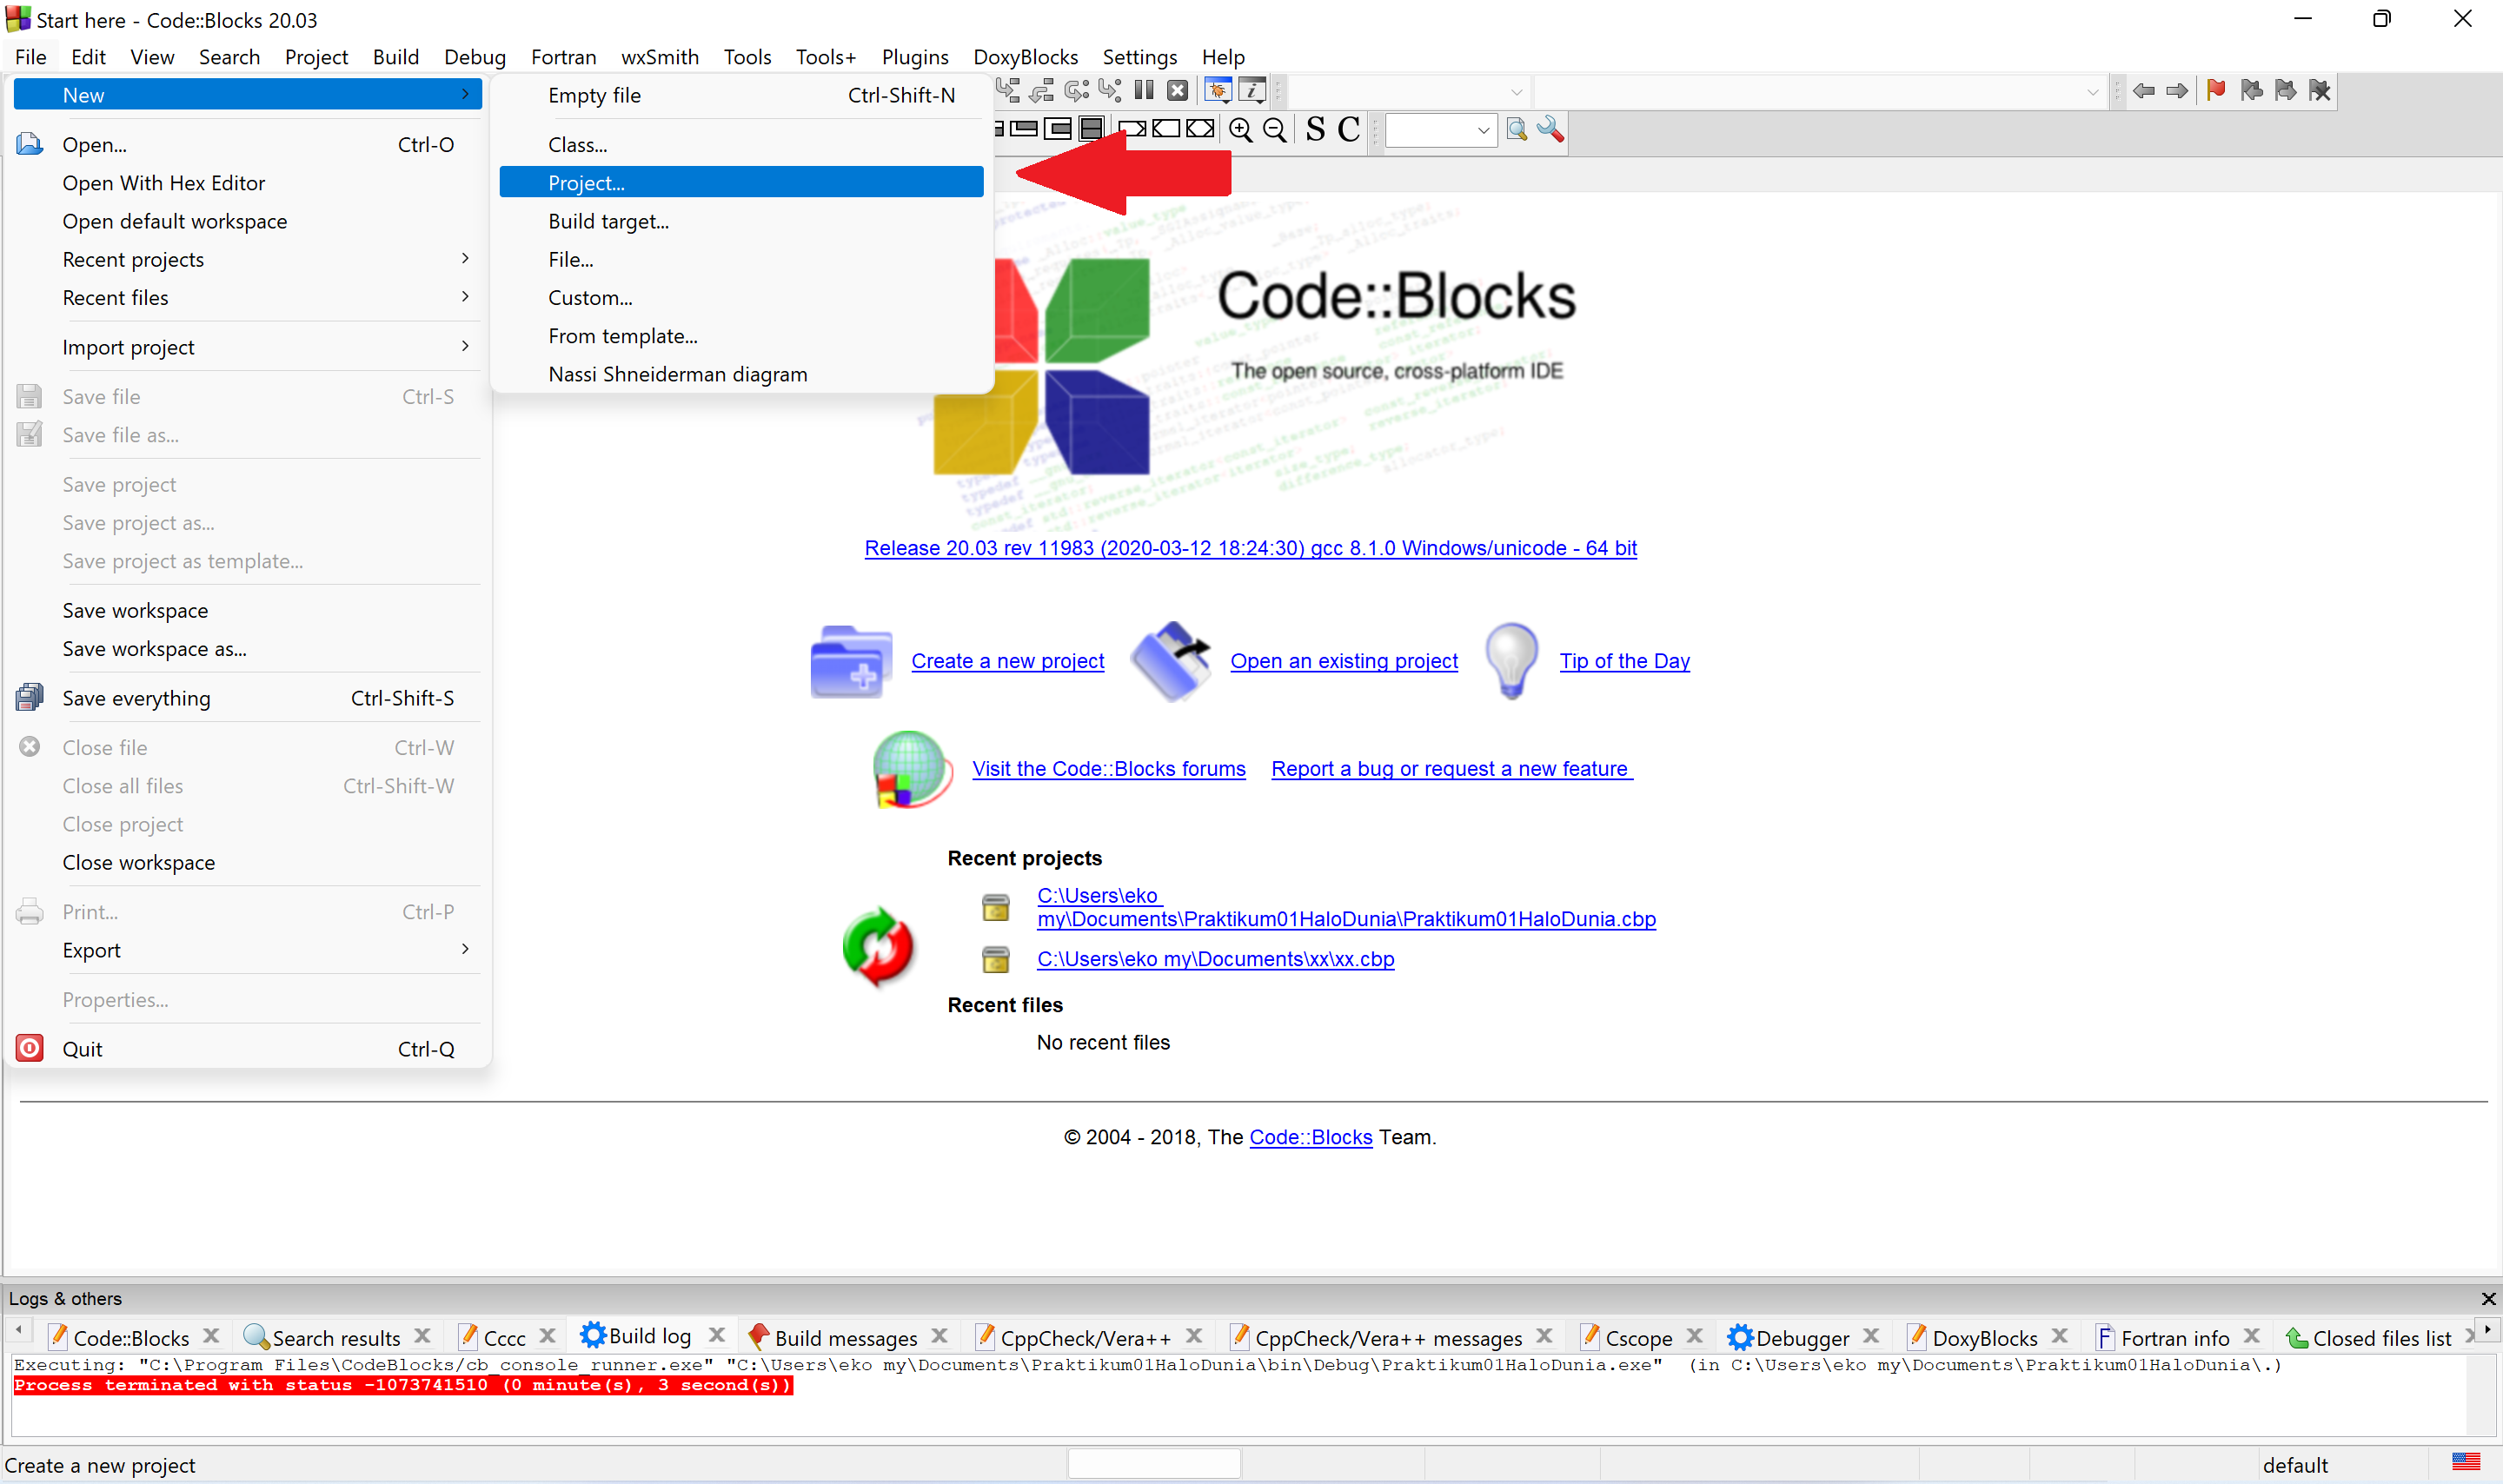
\includegraphics[width=0.7\linewidth]{P1/img/screenshot002.png}
		      \caption{}
		      \label{fig:screenshot002}
	      \end{figure}
	\item Click on Console Application
	      \begin{figure}[H]
		      \centering
		      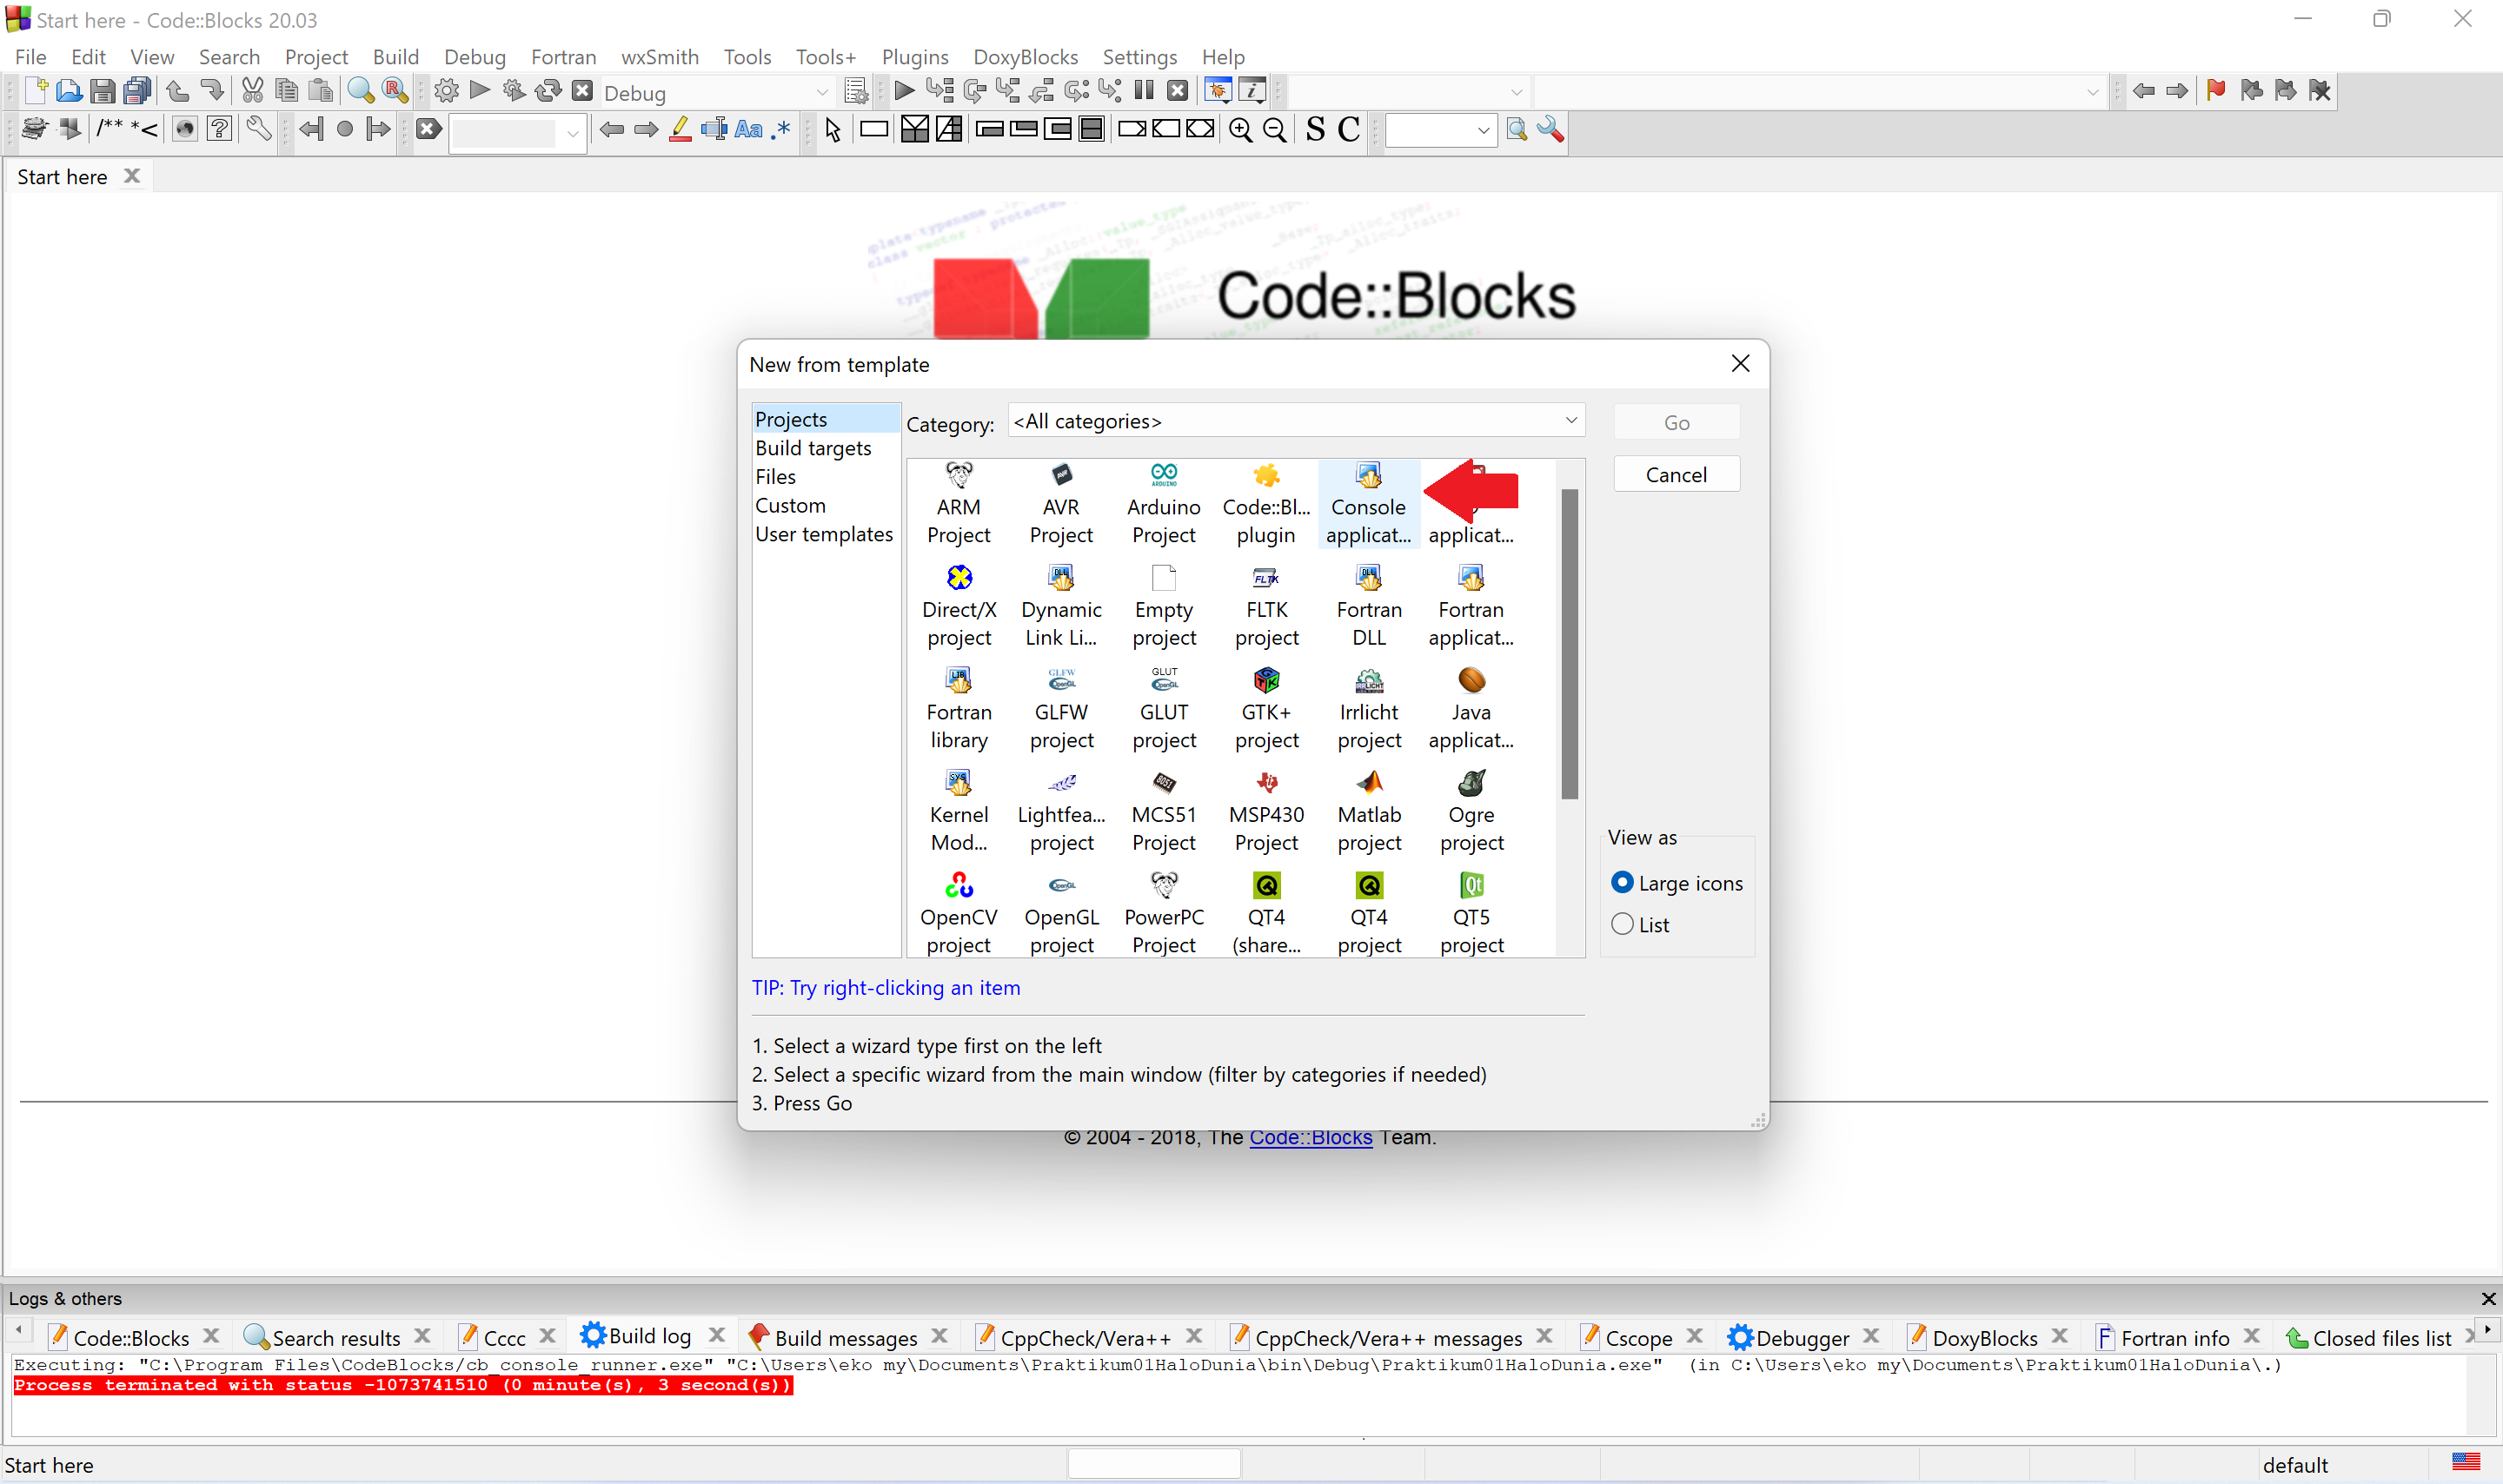
\includegraphics[width=0.7\linewidth]{P1/img/screenshot004.png}
		      \caption{}
		      \label{fig:screenshot004}
	      \end{figure}
	\item Choose C as the programming language
	      \begin{figure}[H]
		      \centering
		      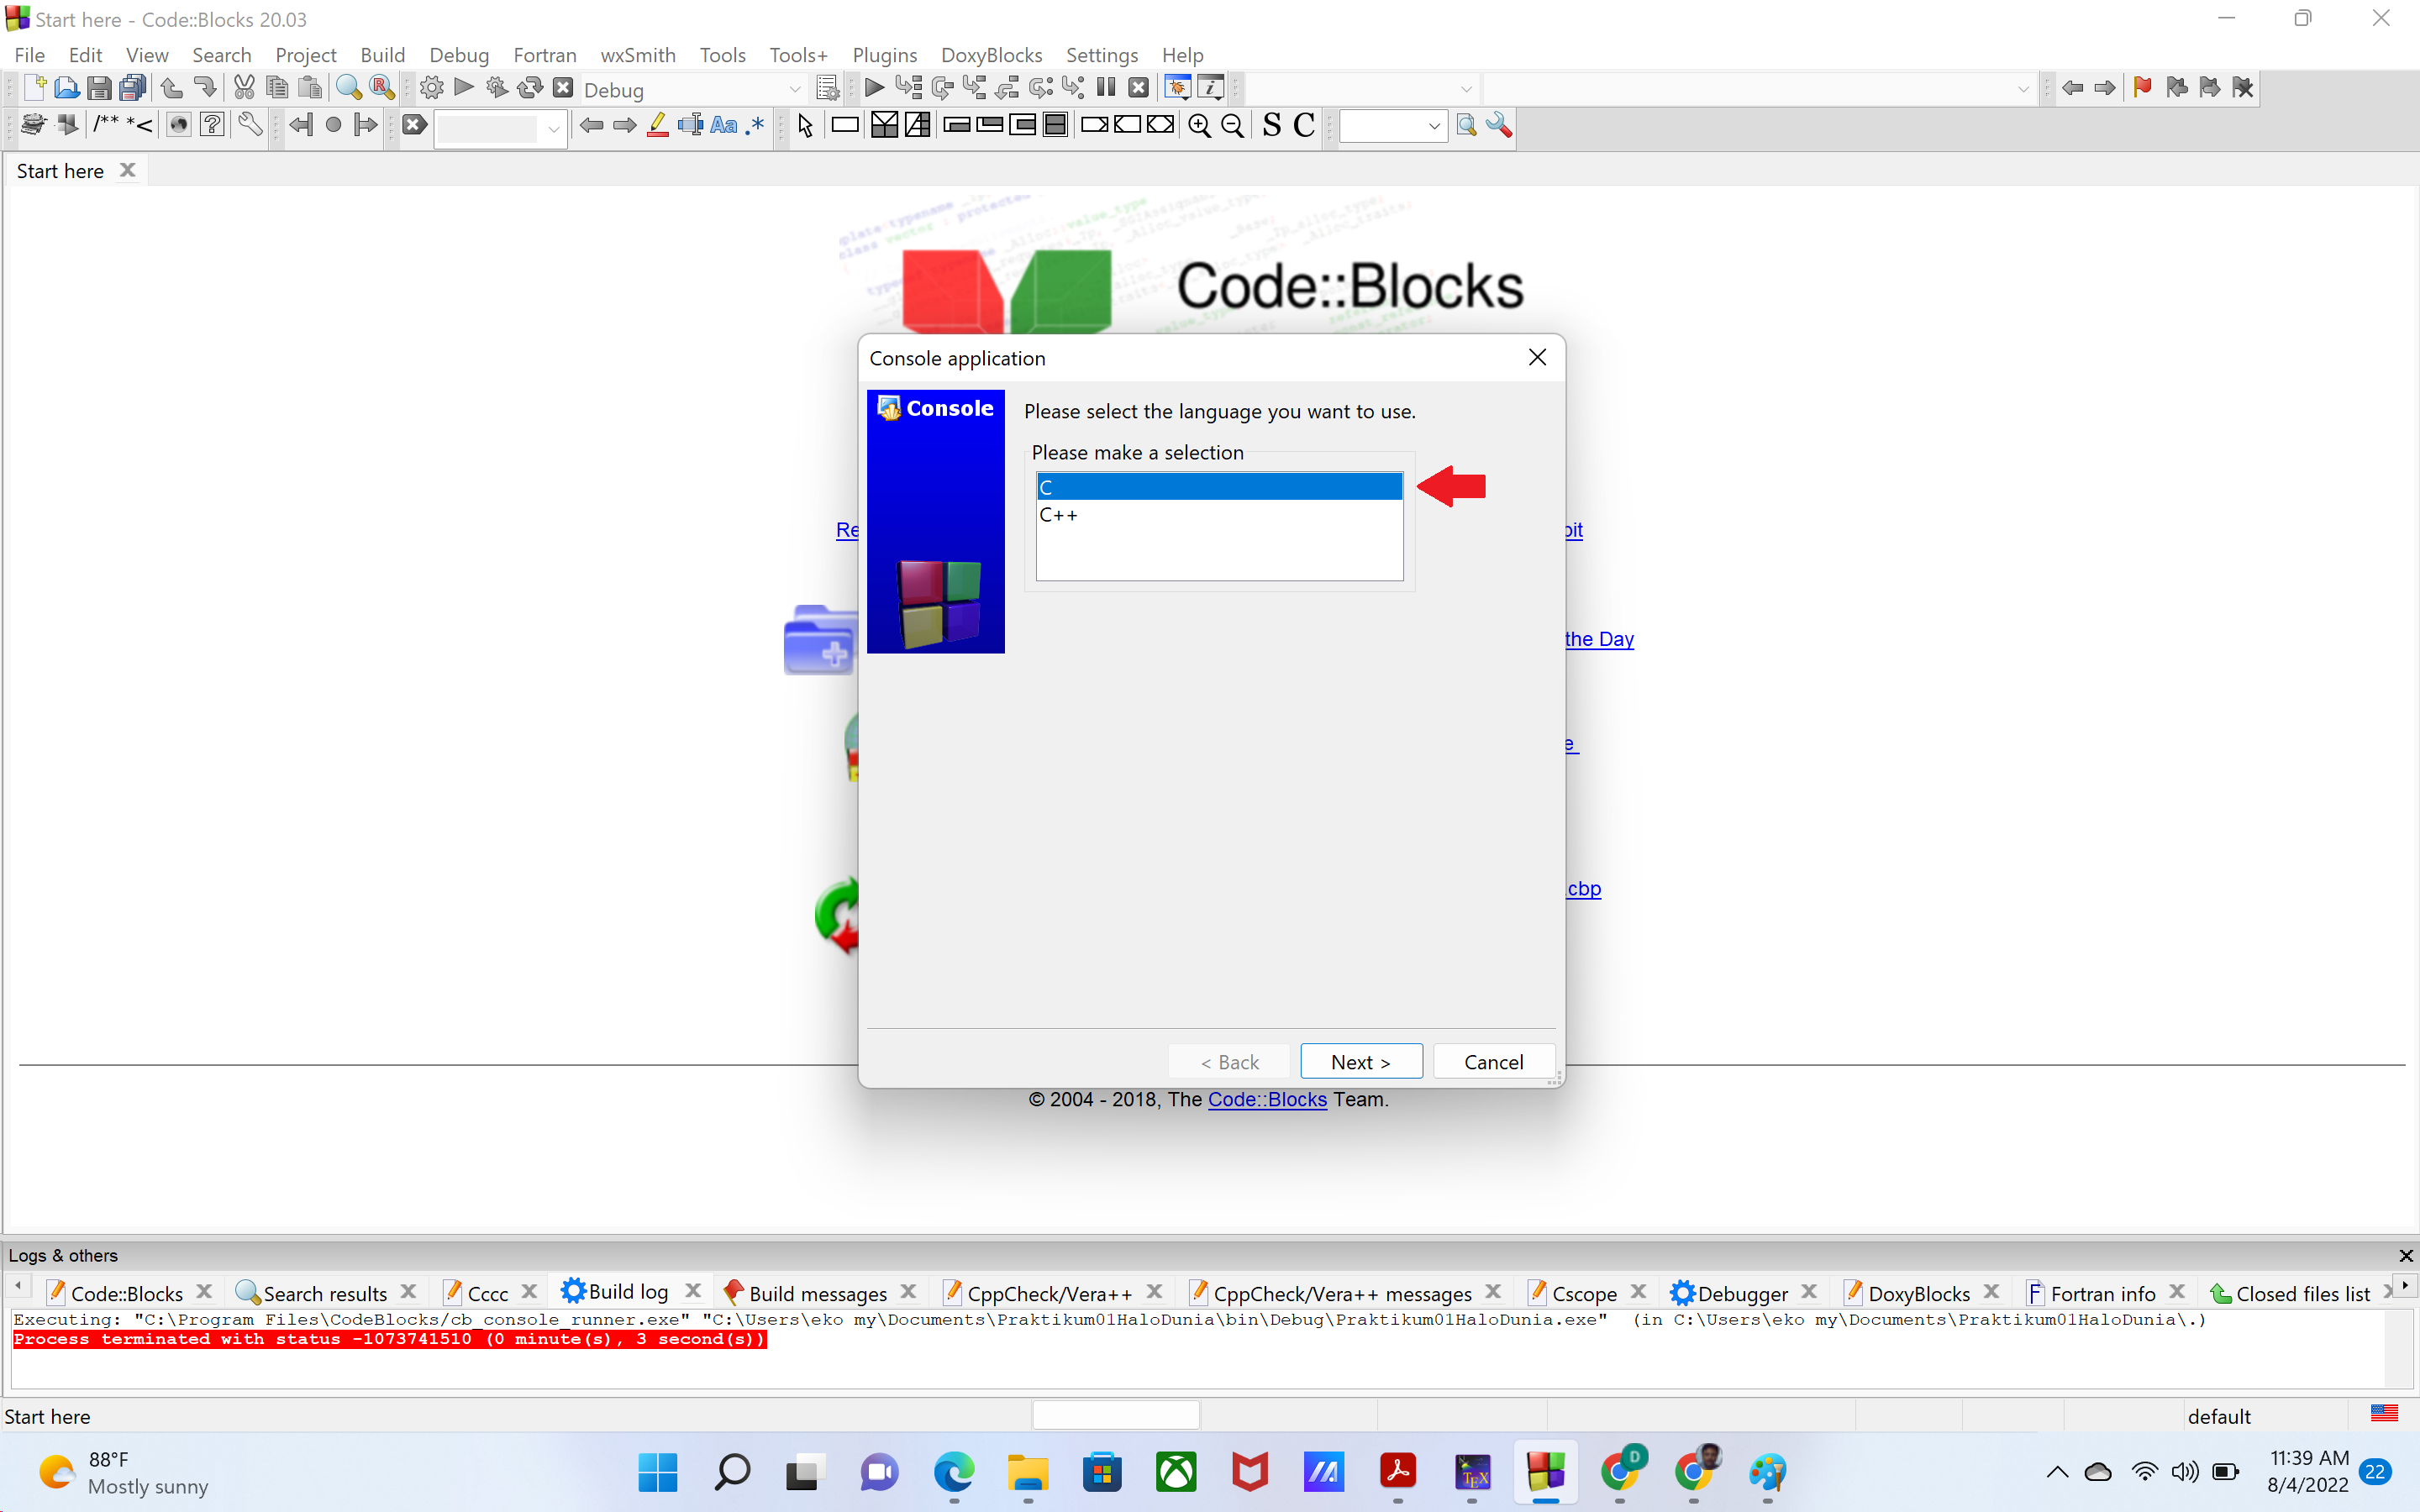
\includegraphics[width=0.7\linewidth]{P1/img/screenshot005.png}
		      \caption{}
		      \label{fig:screenshot005}
	      \end{figure}
	\item Insert your project name
	      \begin{figure}[H]
		      \centering
		      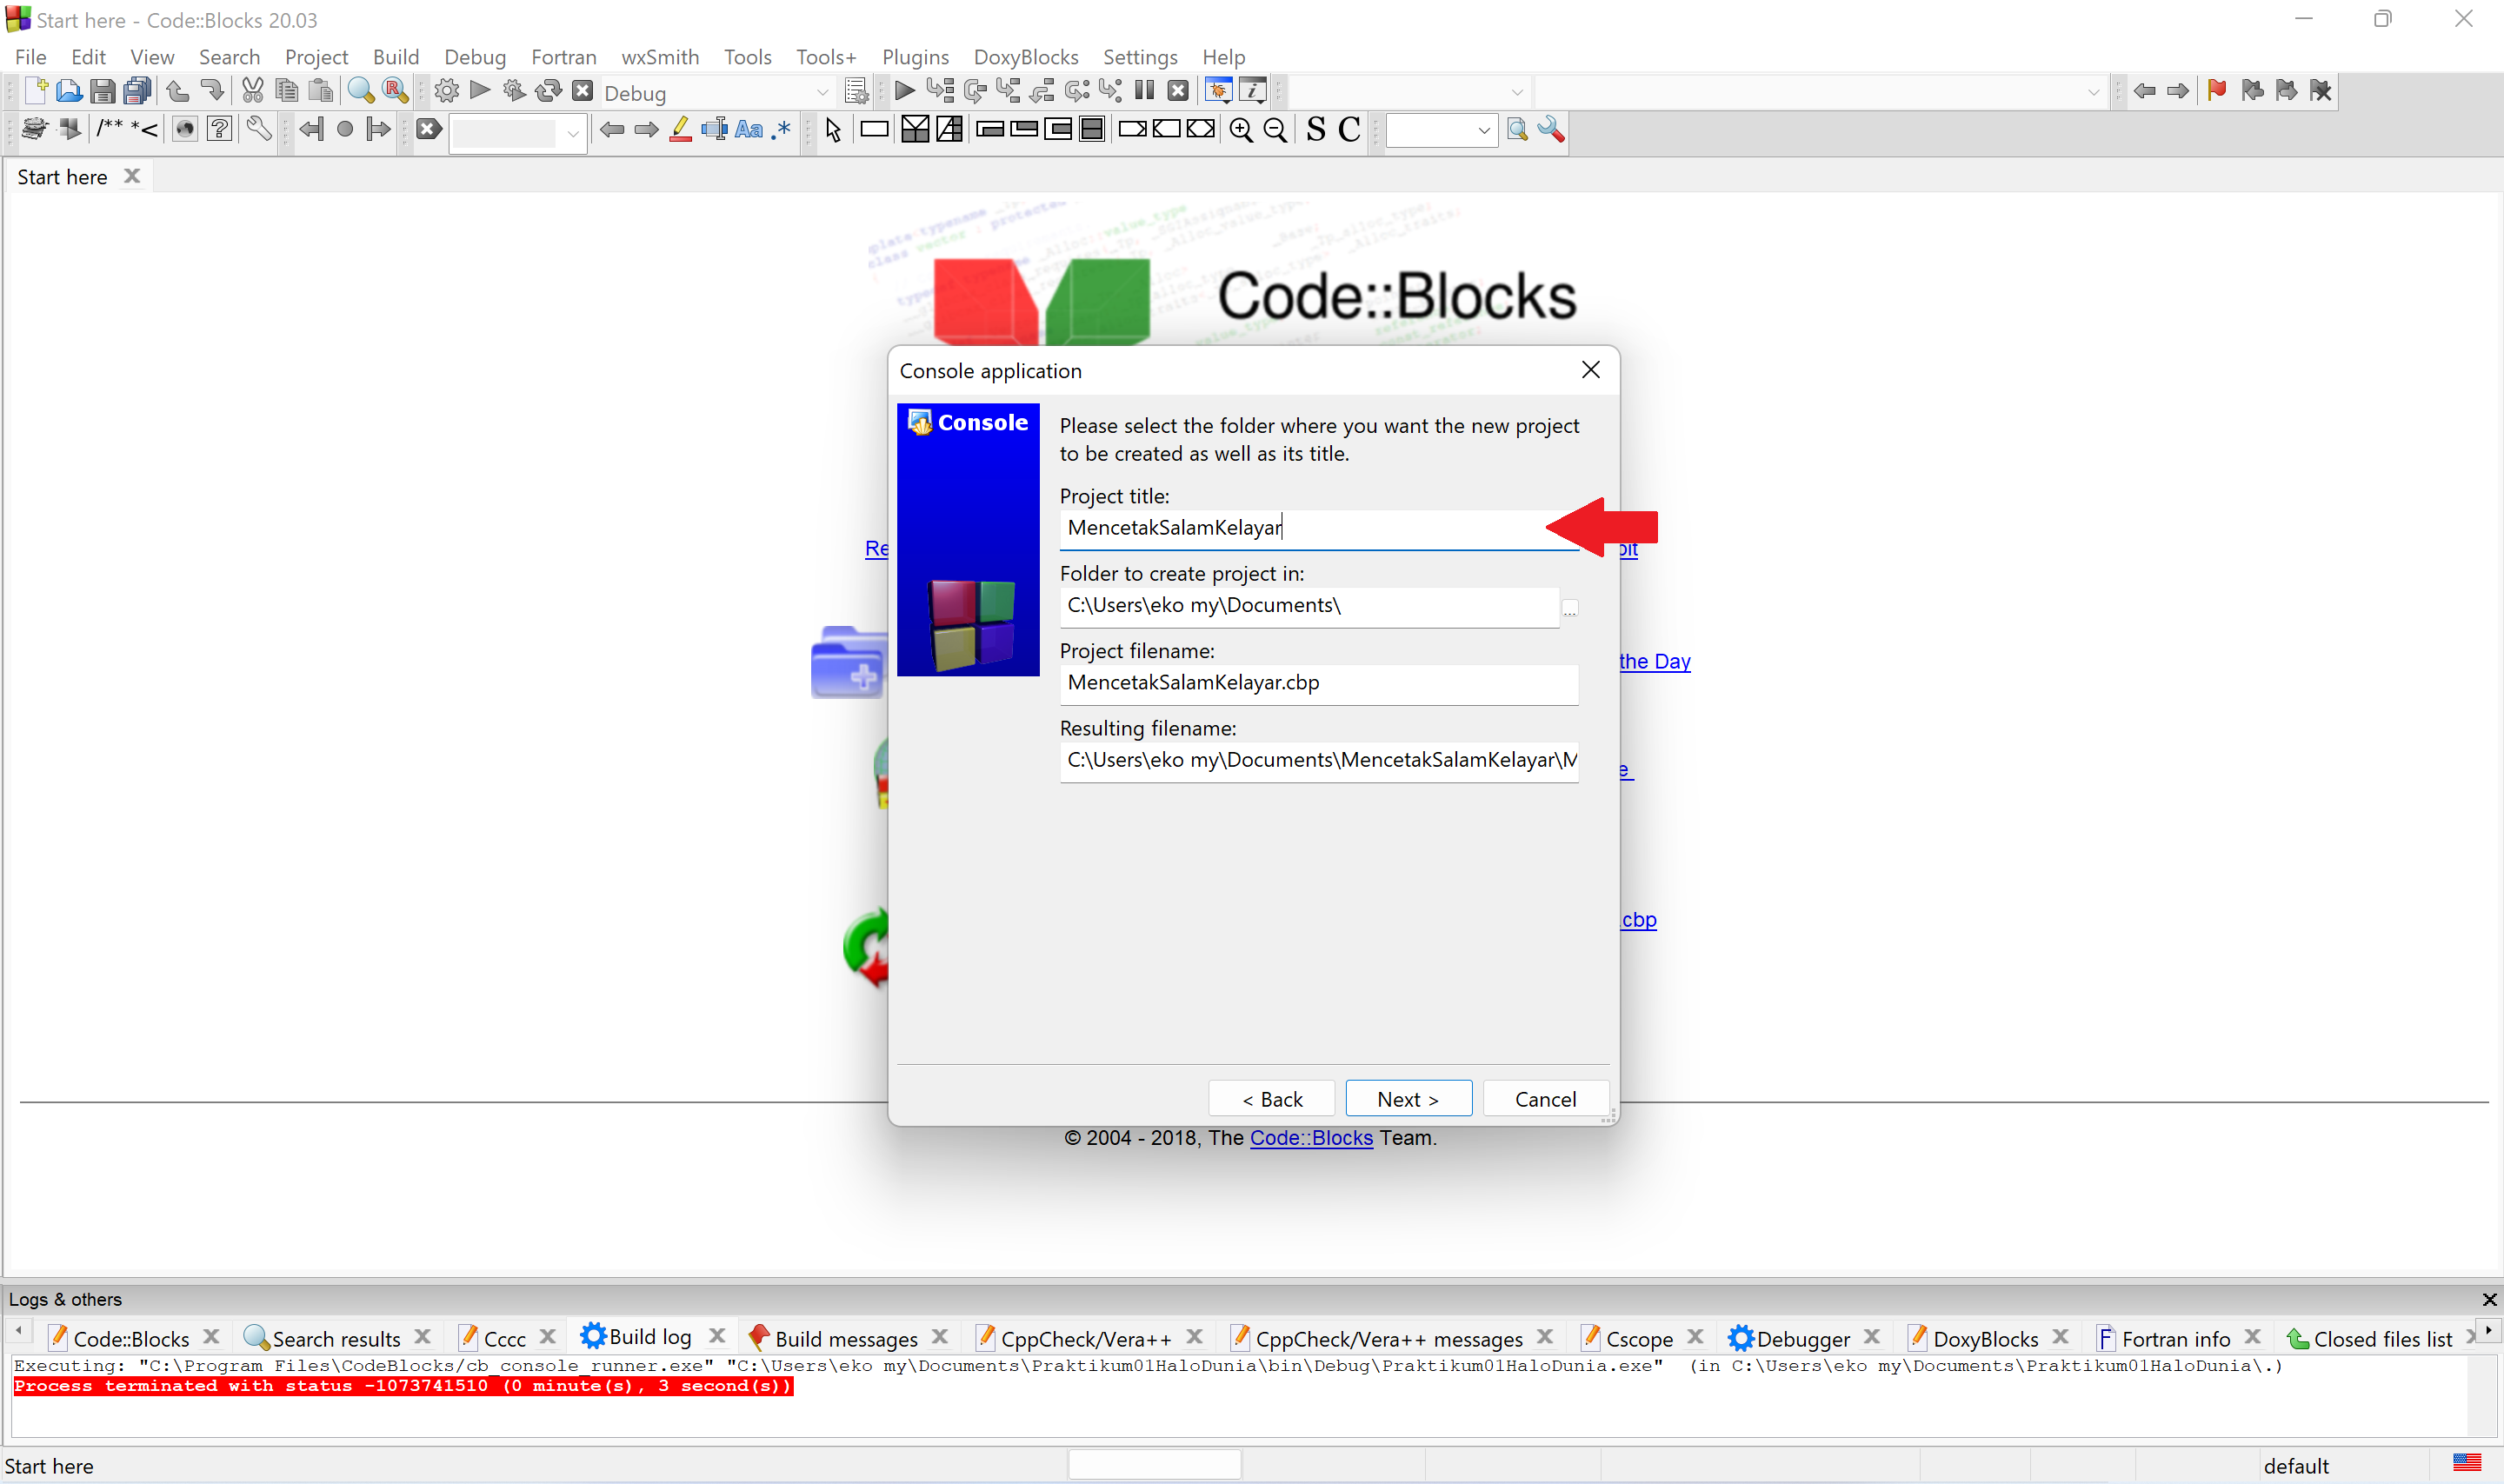
\includegraphics[width=0.7\linewidth]{P1/img/screenshot006.png}
		      \caption{}
		      \label{fig:screenshot006}
	      \end{figure}
	\item Choose the compiler (gcc), select a directory to save your project, and click save
	      \begin{figure}[H]
		      \centering
		      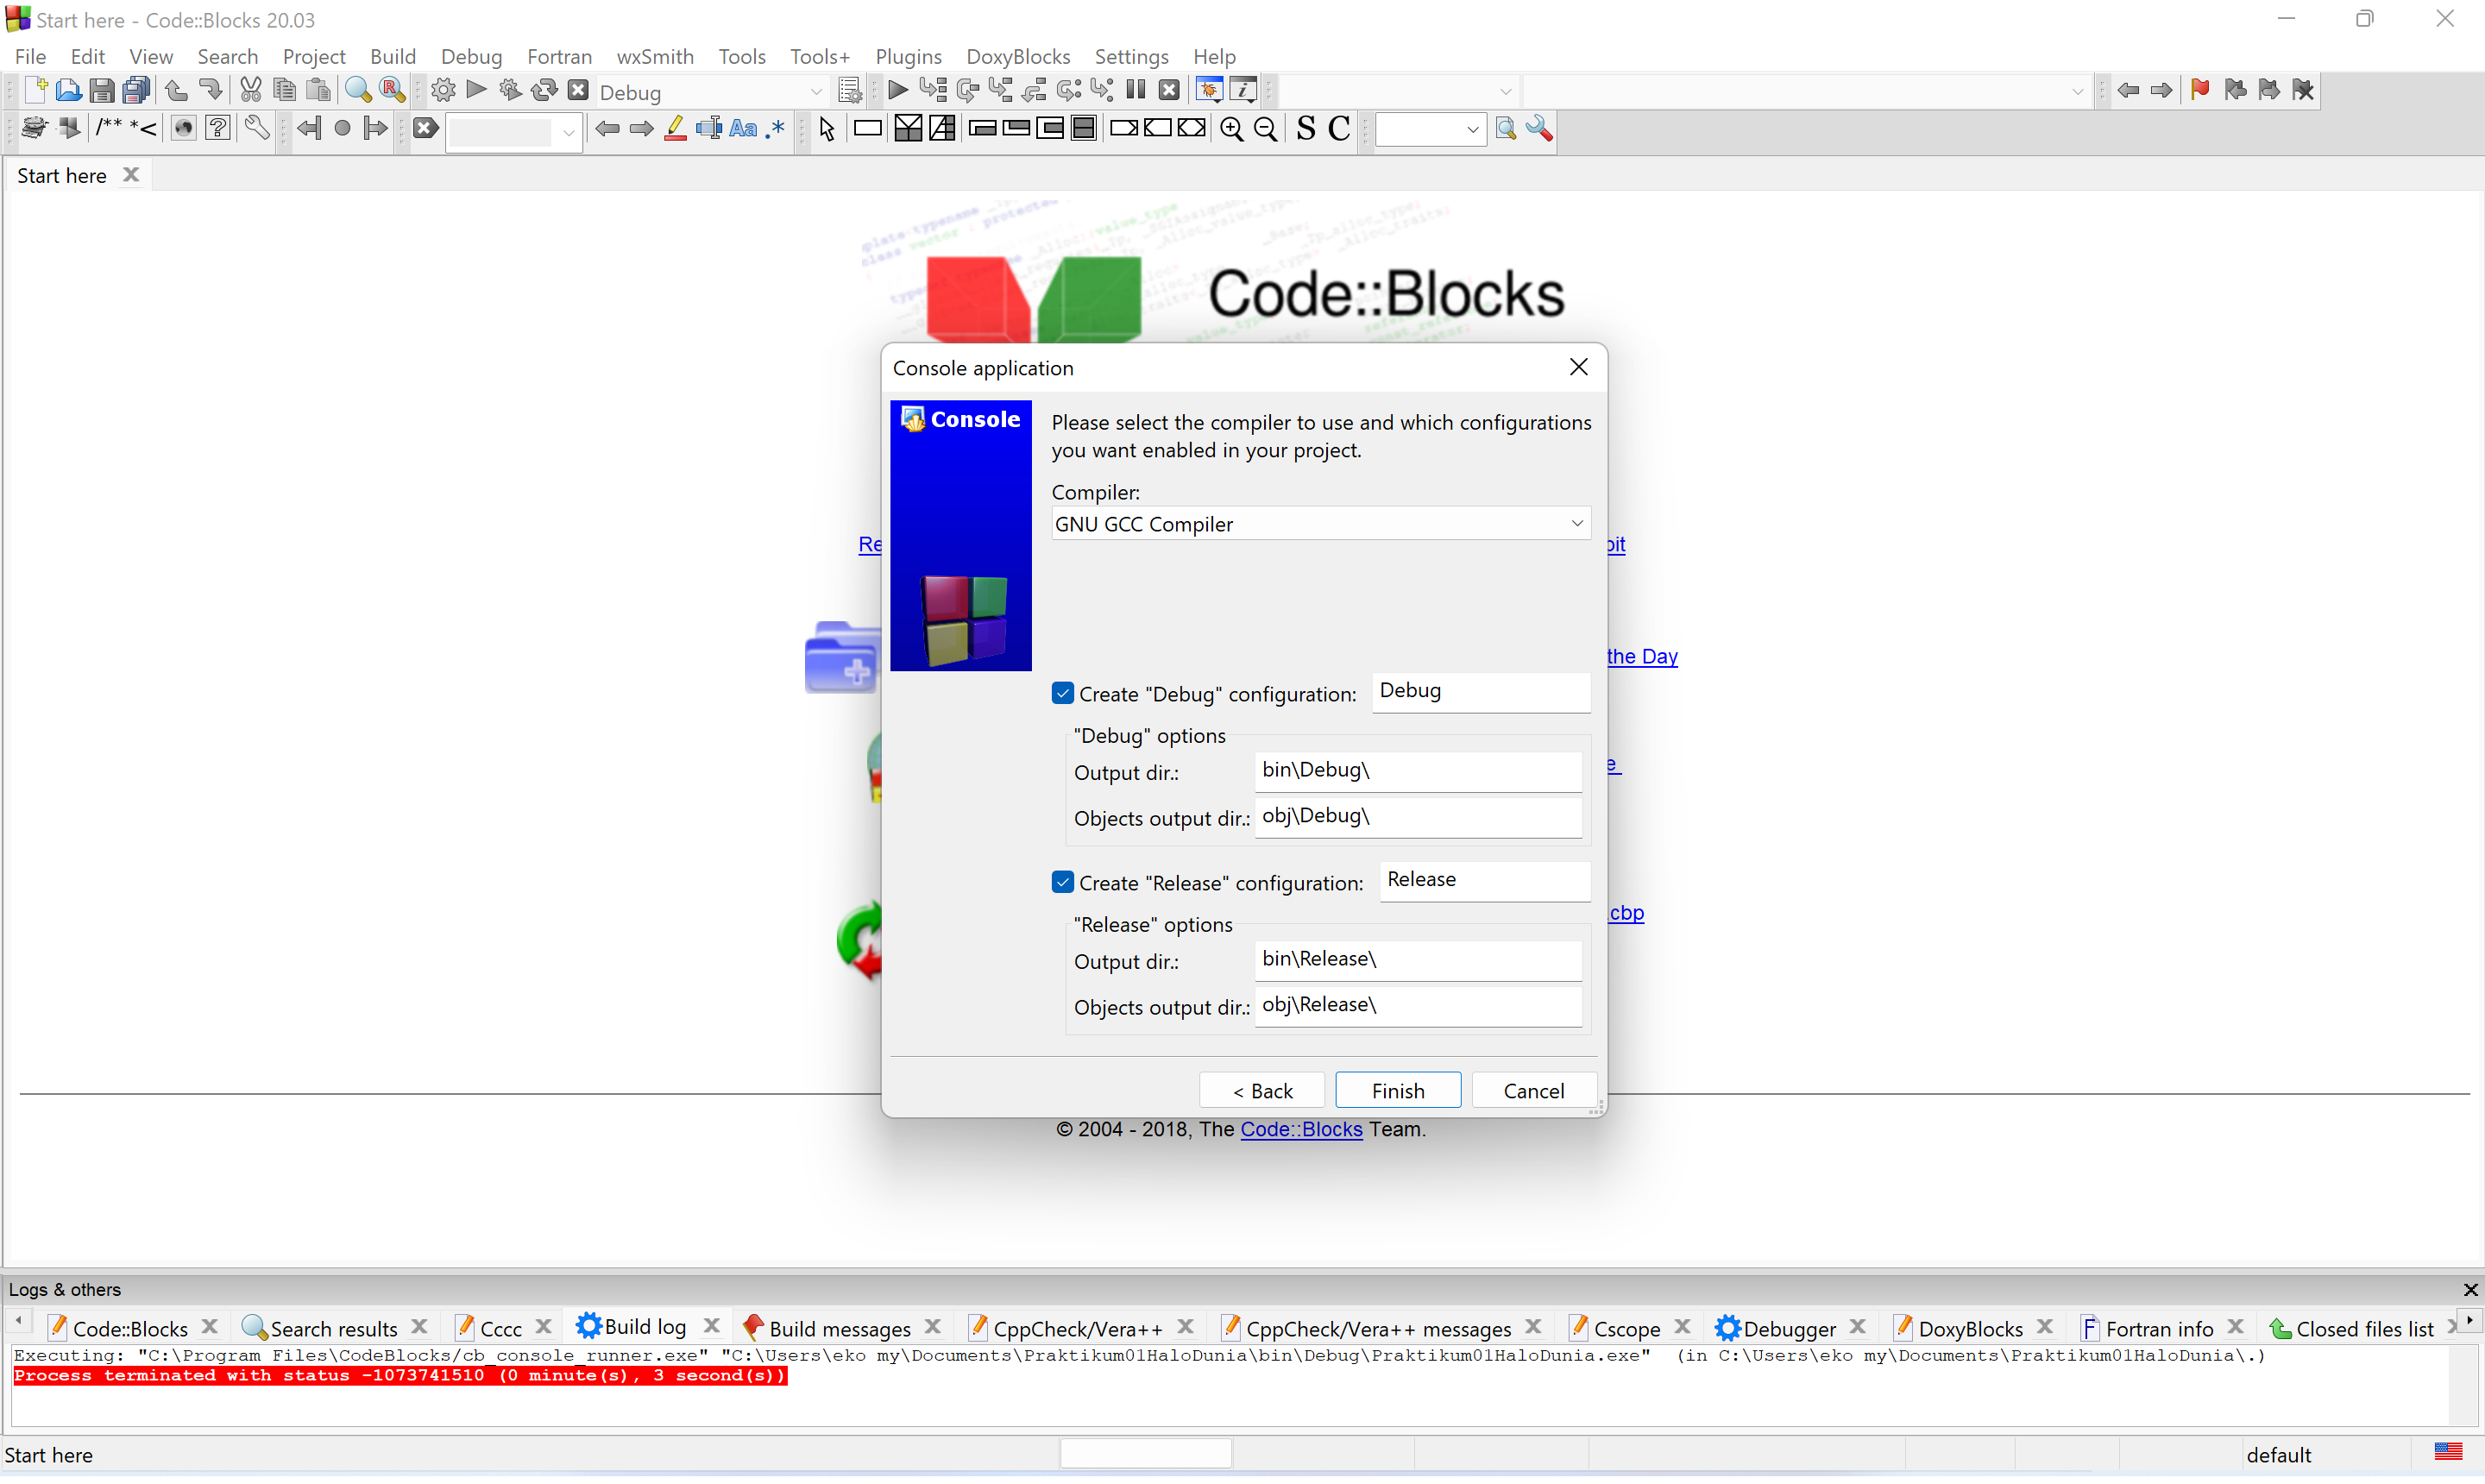
\includegraphics[width=0.7\linewidth]{P1/img/screenshot007.png}
		      \caption{}
		      \label{fig:screenshot007}
	      \end{figure}
	\item Write code as in Figure \ref{fig:screenshot008} in Code::Blocks
	      \begin{figure}[H]
		      \centering
		      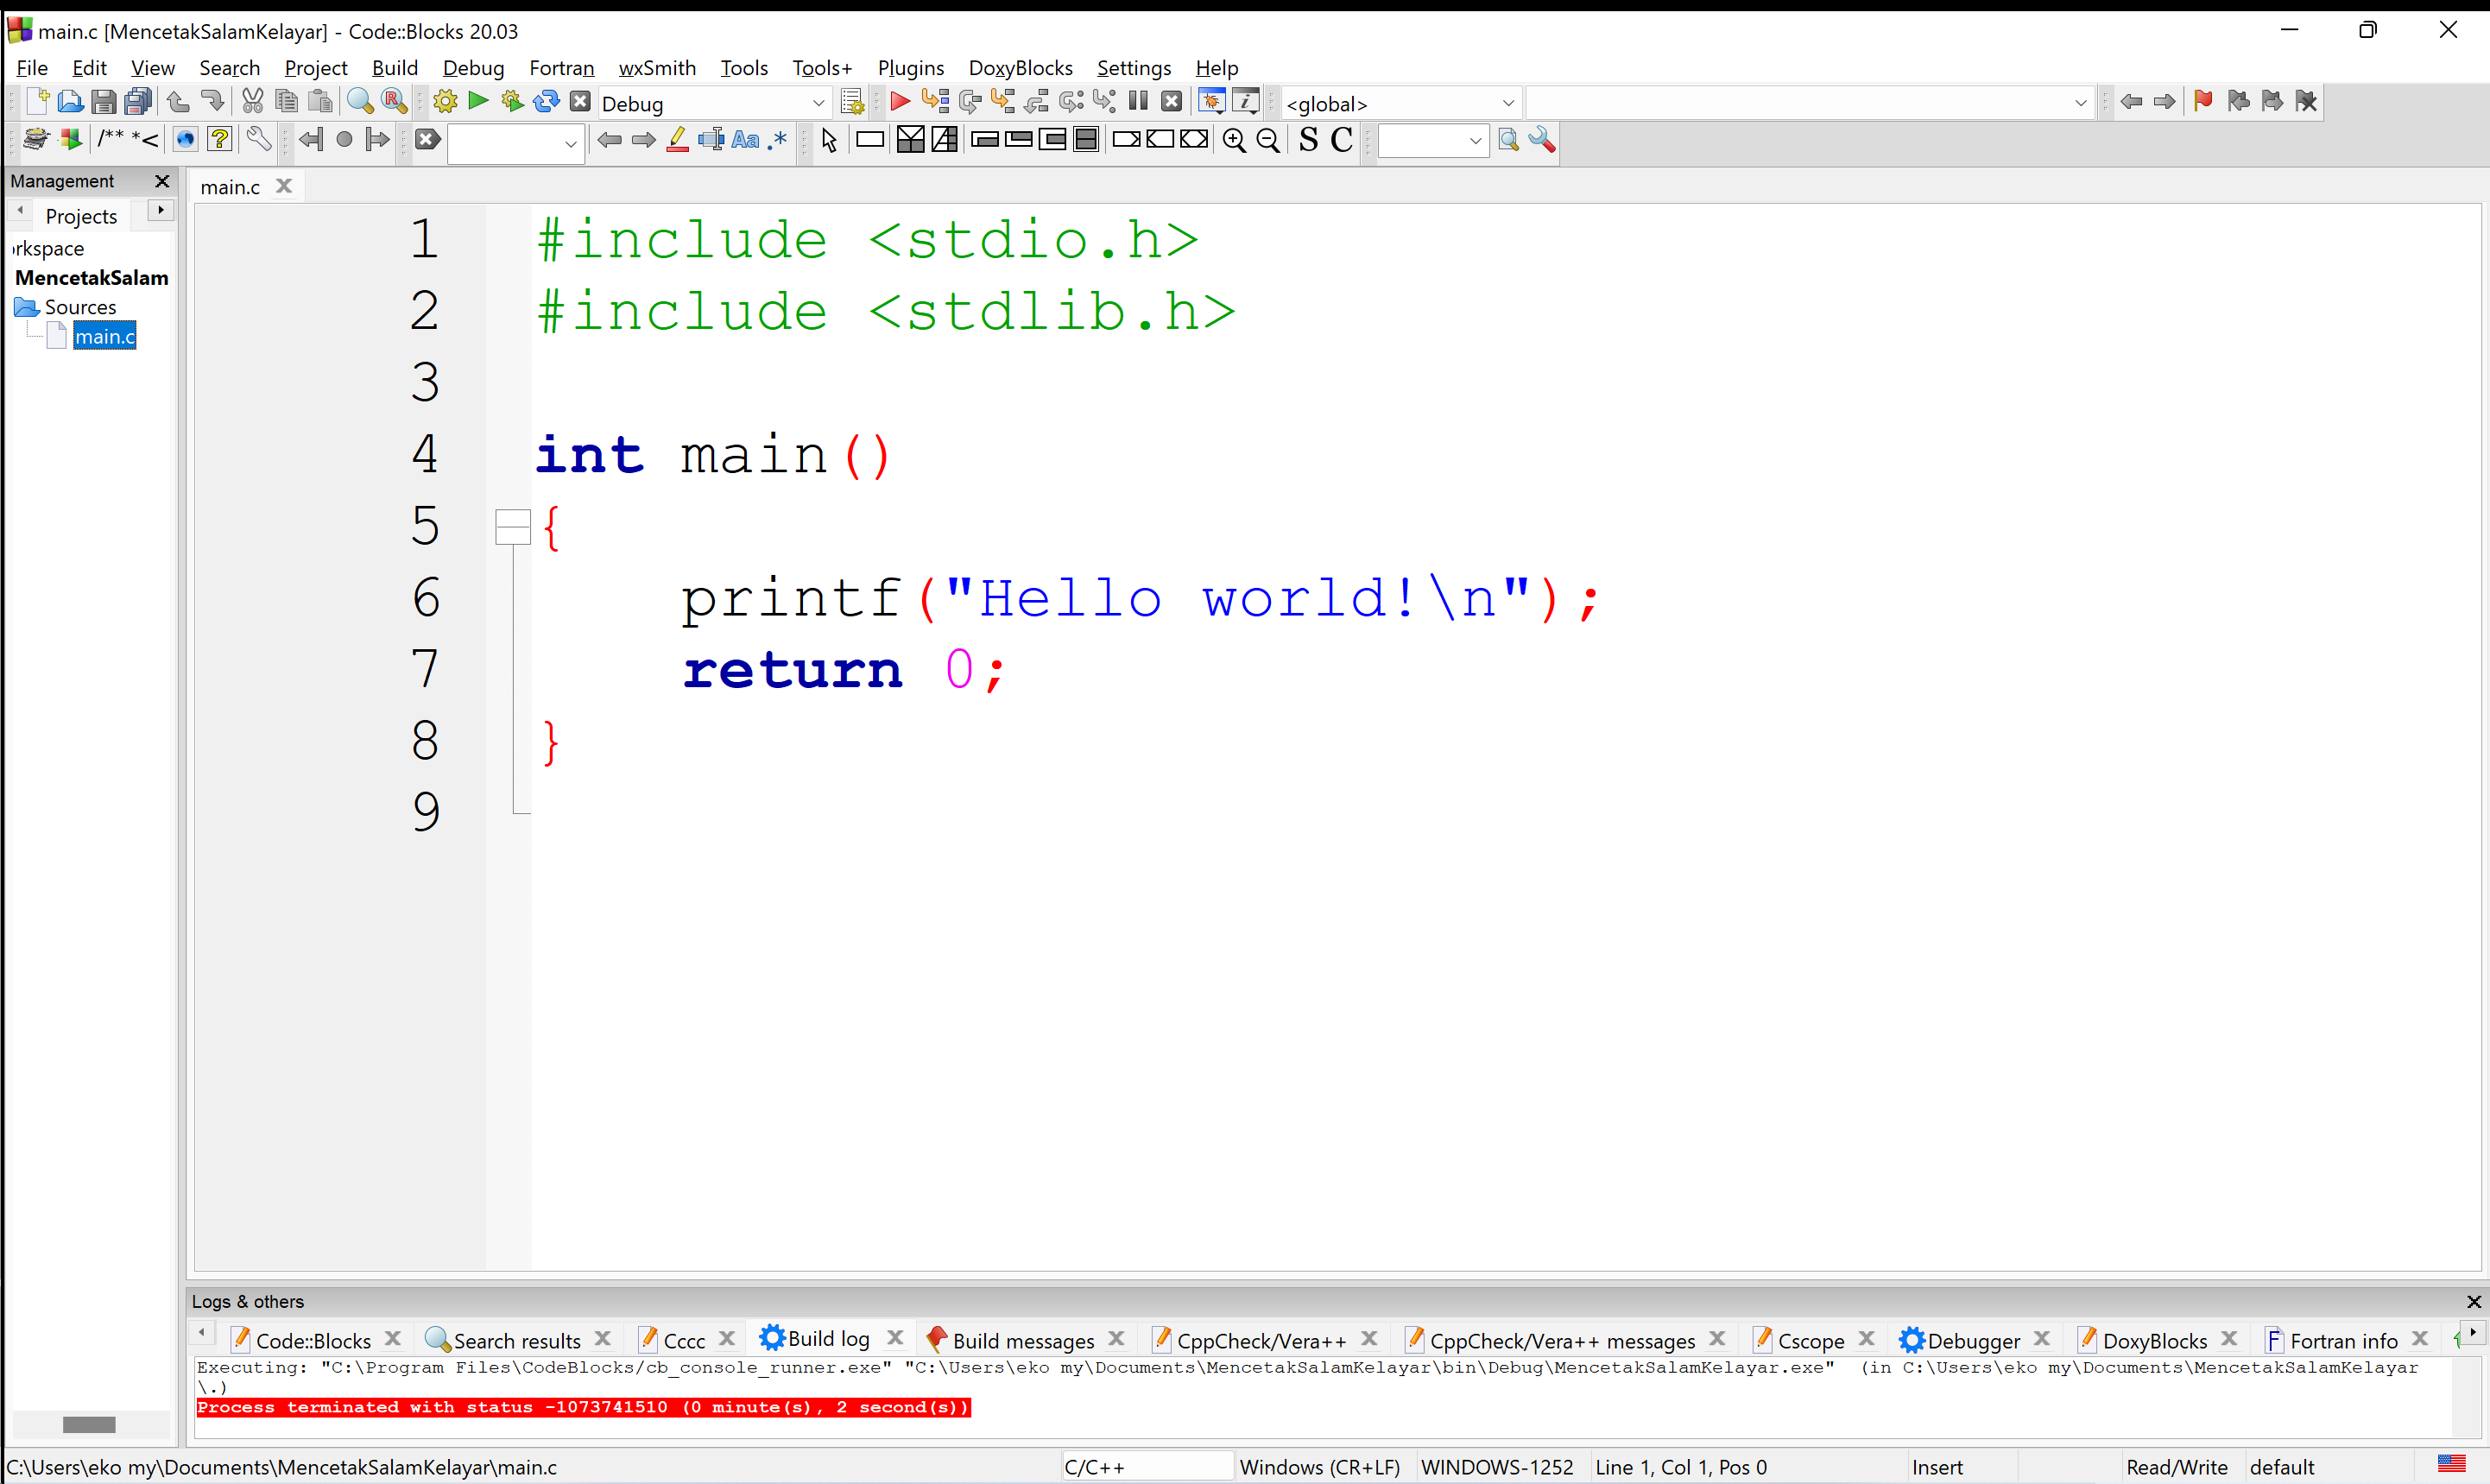
\includegraphics[width=0.7\linewidth]{P1/img/screenshot008.png}
		      \caption{}
		      \label{fig:screenshot008}
	      \end{figure}
	\item Click Build$->$Build and Run or press F9 on your keyboard
	      \begin{figure}[H]
		      \centering
		      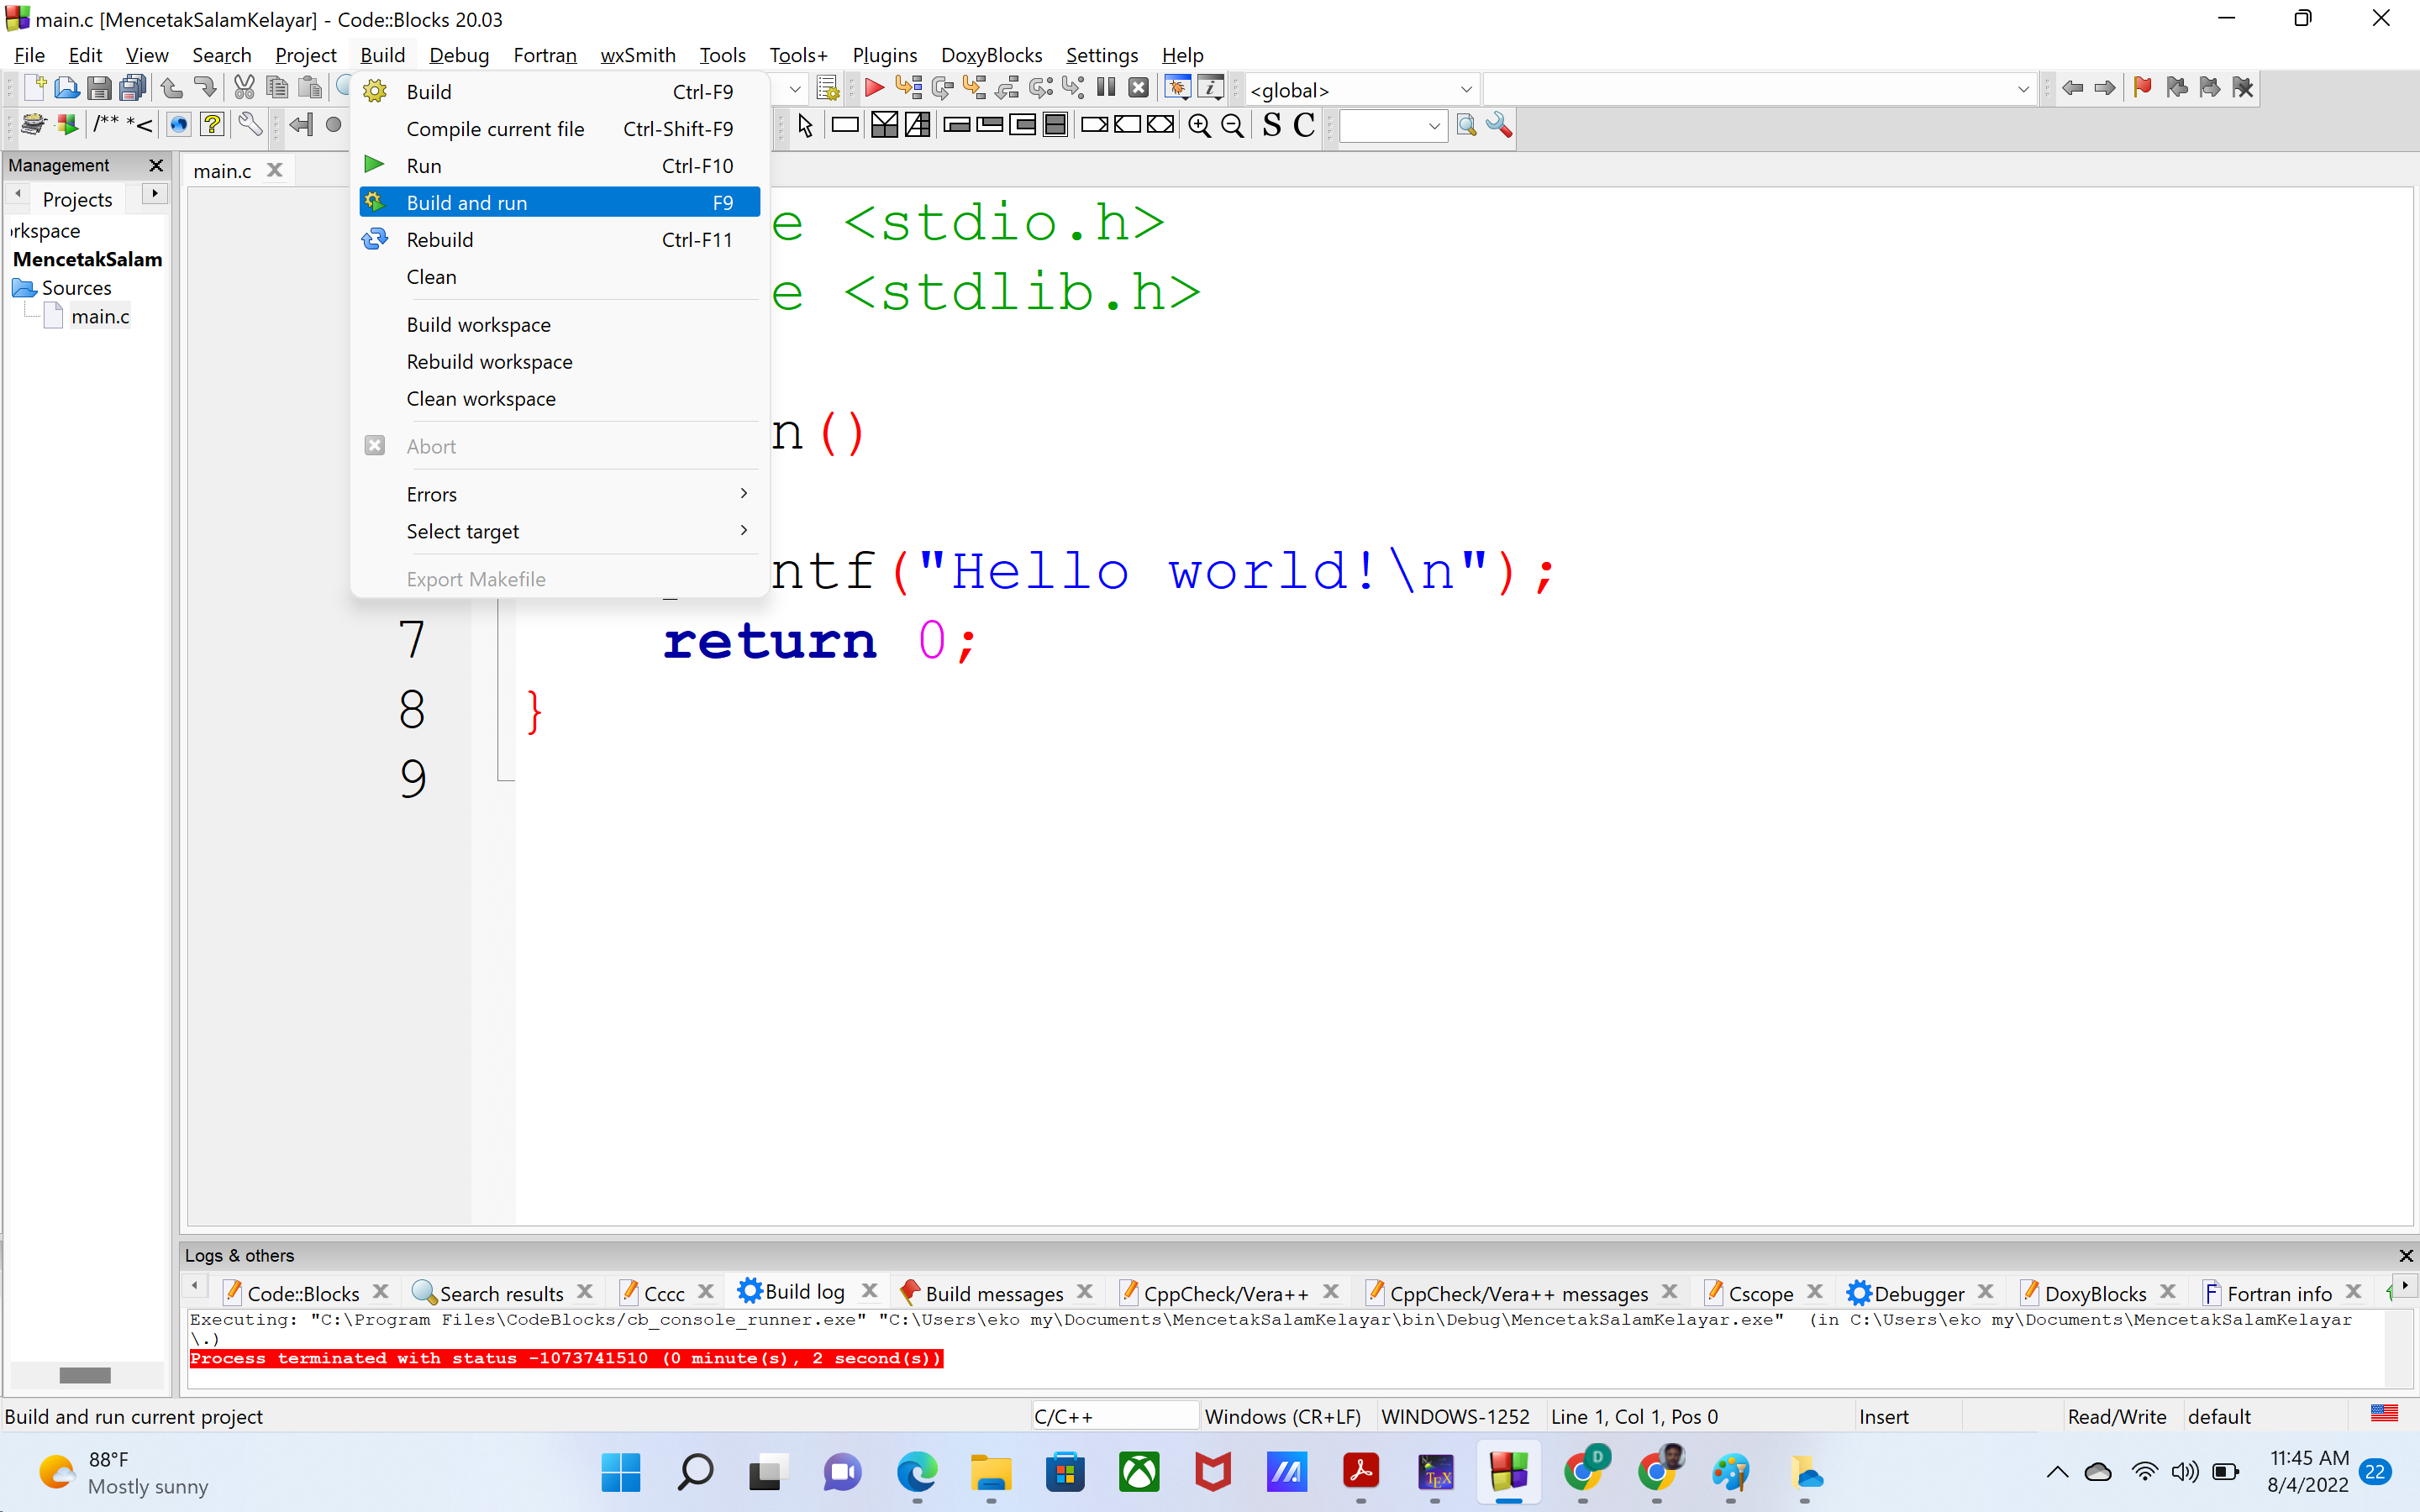
\includegraphics[width=0.7\linewidth]{P1/img/screenshot009.png}
		      \caption{}
		      \label{fig:screenshot009}
	      \end{figure}
	      % \item The program outputs can be seen on the console.
	\item The program output can be seen on the console tab
	      \begin{figure}[H]
		      \centering
		      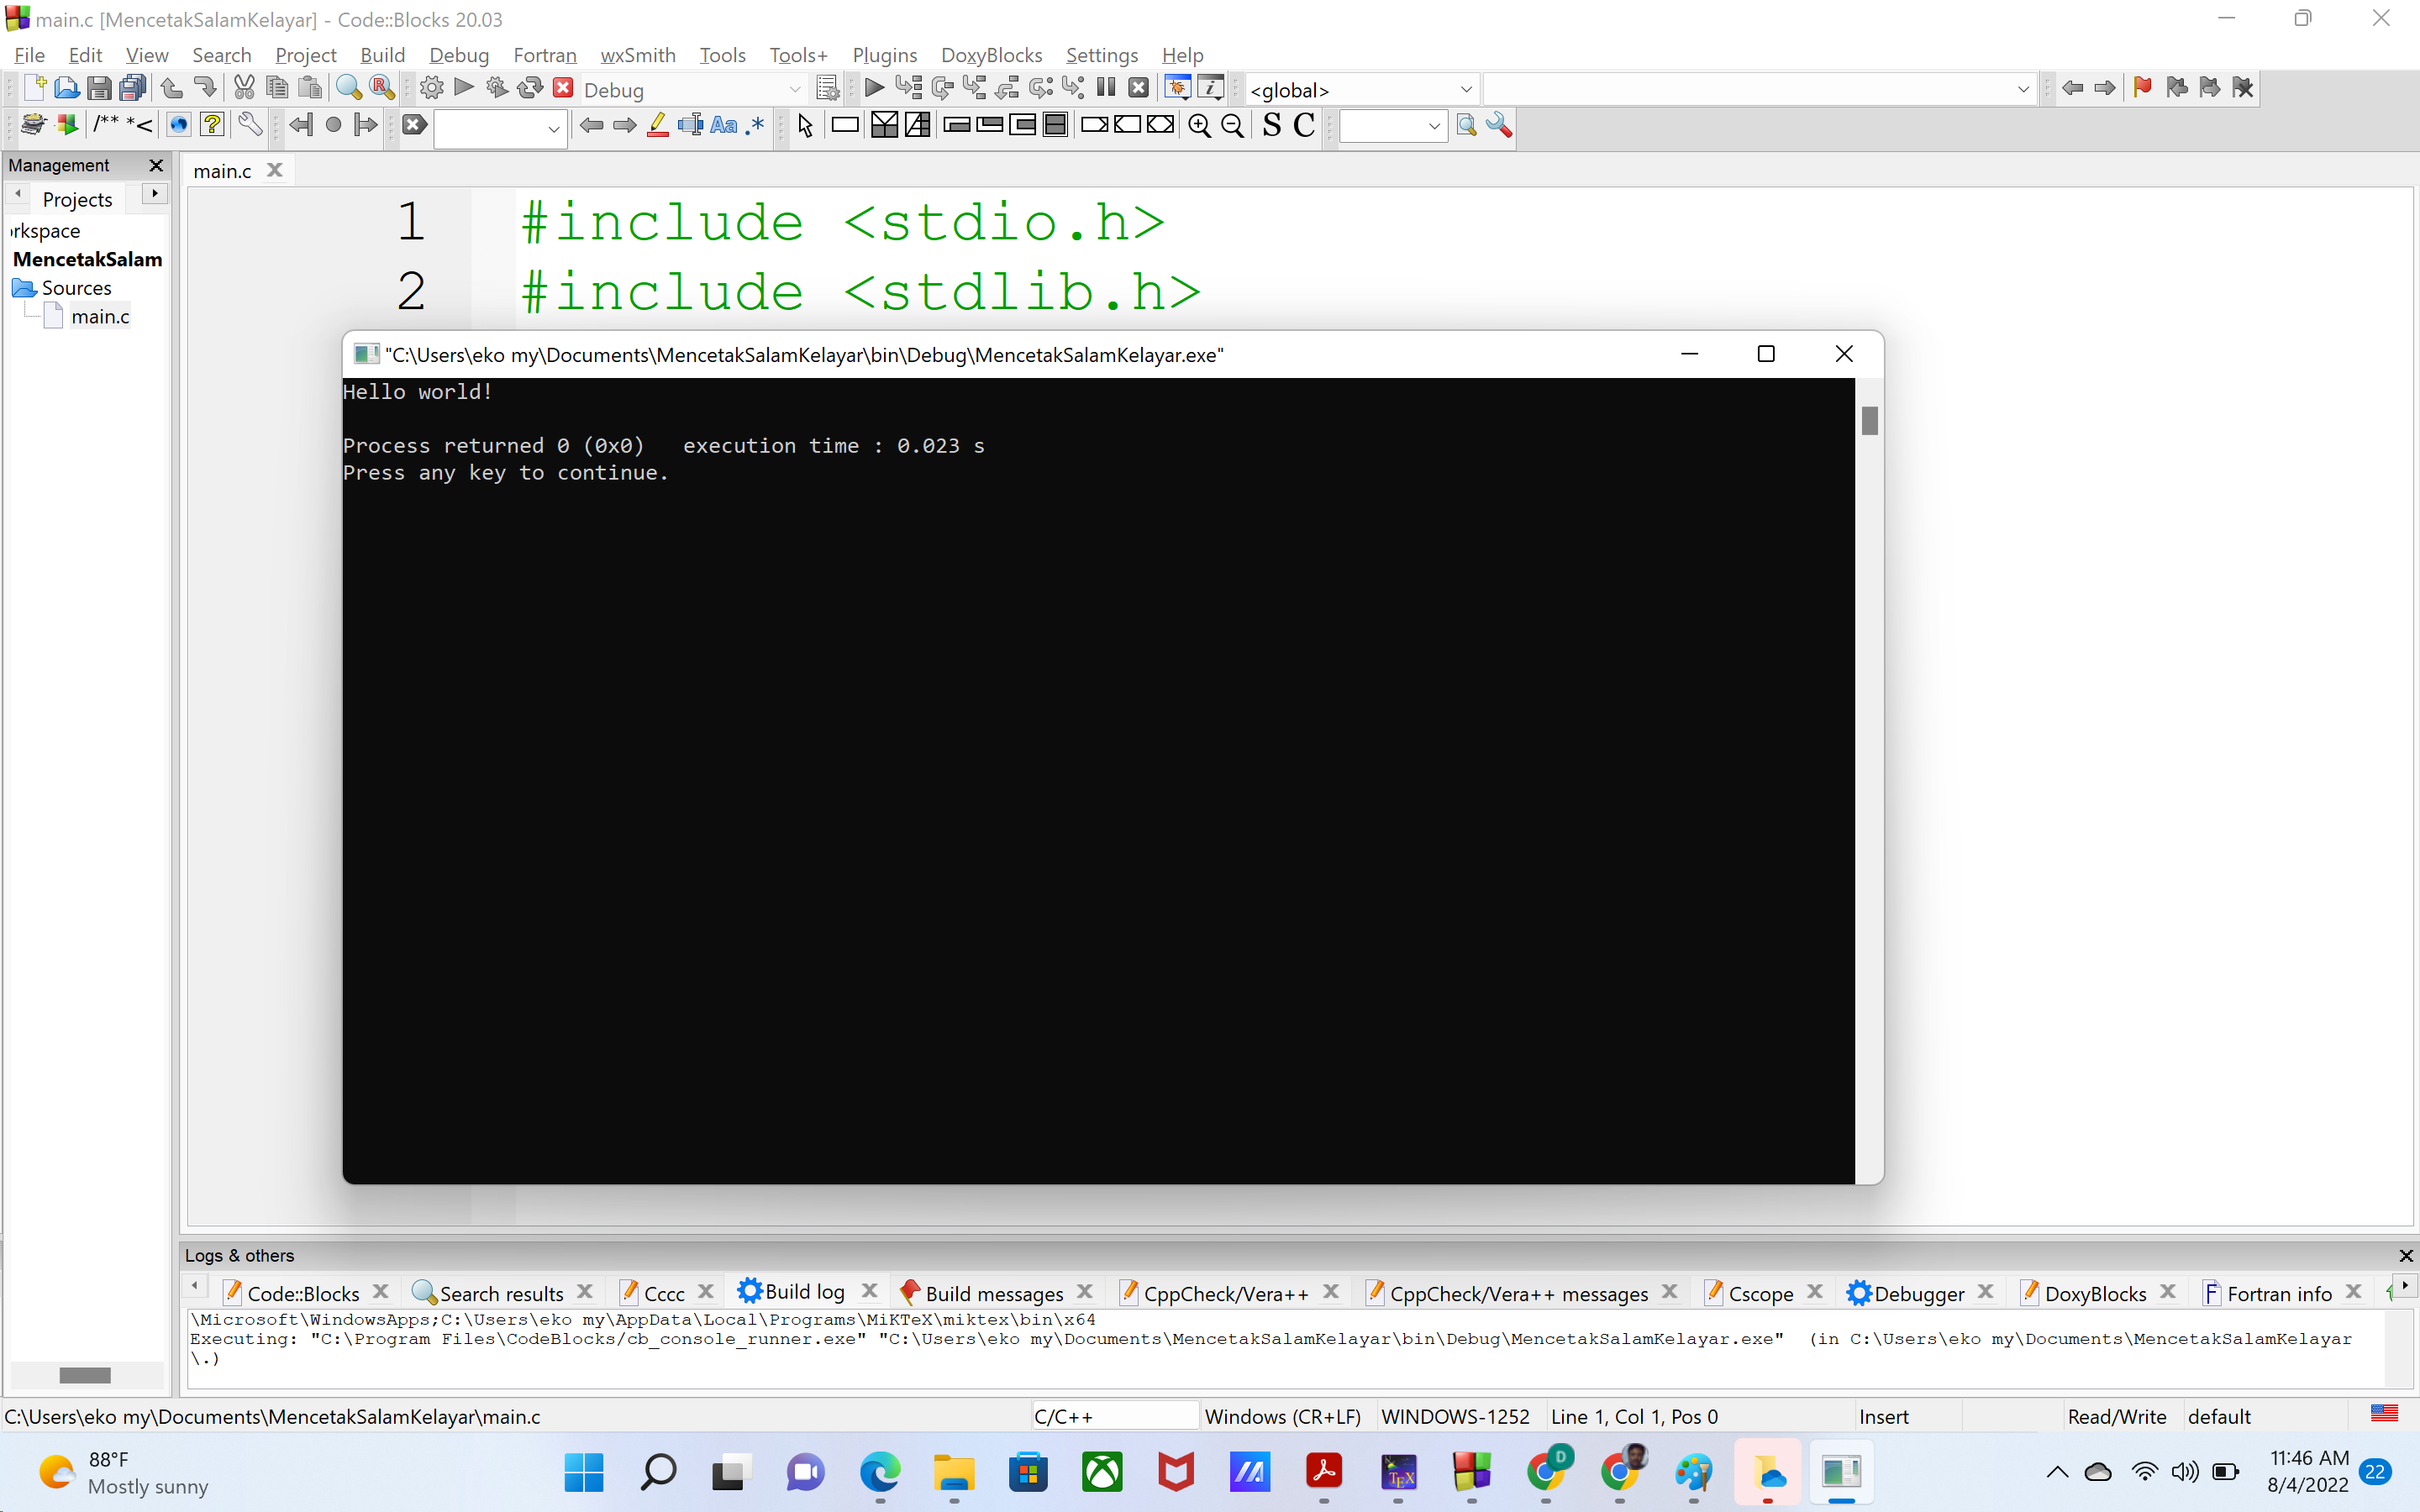
\includegraphics[width=0.7\linewidth]{P1/img/screenshot010.png}
		      \caption{}
		      \label{fig:screenshot010}
	      \end{figure}
\end{enumerate}

\section{Structure of C Language}

\begin{lstlisting}[language=c,caption=Simple example program in C,label=lst:helloworld,captionpos=t]
	#include <stdio.h>

	int main() {
		printf("Hello World!");
		return 0;
	}
\end{lstlisting}
Here is the explanation of the code above:
\begin{enumerate}
	\item \verb|#include <stdio.h>|
	This is a header file where we include the functions inside 'stdio.h', which contains basic input and output functions such as printf().
	
	\item int main()
	This is the main function. It must exist in every C program.  
	All code inside the curly braces \{\} will be executed when the program runs.
	
	\item printf("Hello World!");
	This is a function to output "Hello World!".  
	Notice that at the end there is a semicolon ';'. Every statement in C must end with a semicolon.
	
	\item return 0;
	This is a statement that returns a value to the main() function.  
	The function ends when this return is executed. Any code written below it, even if still inside the curly braces, will be ignored.
\end{enumerate}
C ignores whitespace, so the program above could also be written as:
\begin{lstlisting}[language=c]
	int main(){printf("Hello World!");return 0;}
\end{lstlisting}
However, writing it this way makes the code harder to read.  
It is better to write the program with spaces and on separate lines to make it easier to understand.

\subsection*{Pre-Lab Assignment 1}
\begin{enumerate}
	\item From the example above, what happens if \verb|#include <stdio.h>| is removed?
  	\item If the code is written as below, what will happen? Why does that occur?
	\begin{lstlisting}[language=c]
	#include <stdio.h>

	int main() {
		return 0;
		printf("Hello World!");
	}
\end{lstlisting}
\end{enumerate}

\section{Data Types}

In the C language, there are 3 basic data types: int (integer), float, and char (character).

\subsection{Integer}

The integer data type stores whole numbers (no decimals).\\
\begin{center}
	\captionof{table}{Integer Data Types \label{tab:integer}}
	\begin{tabular}{|l|c|l|}
		\hline
		\textbf{Type} & \textbf{Size (bytes)} & \textbf{Description} \\ \hline
		int 		& 4 		& basic integer type \\ \hline
		short 		& 2 		& stores smaller integers \\ \hline
		long 		& 4 or 8 	& stores larger integers, depends on the system \\ \hline
		long long 	& 8 		& can store very large numbers \\ \hline
	\end{tabular}
\end{center}

\subsection{Float}

The float data type stores decimal numbers.
\begin{center}
	\captionof{table}{Float Data Types \label{tab:float}}
	\begin{tabular}{|l|c|l|}
		\hline
		\textbf{Type} & \textbf{Size (bytes)} & \textbf{Description} \\ \hline
		float 		& 4 	& sufficient precision for general use \\ \hline
		double 		& 8 	& higher precision, suitable for scientific calculations \\ \hline
		long double	& 10 	& higher precision than double, depends on the compiler \\ \hline
	\end{tabular}
\end{center}

\subsection{Character}

This data type stores characters, such as letters 'a', 'b', 'c', or symbols '@', '\$', '?' etc.
\begin{center}
	\captionof{table}{Char Data Type \label{tab:char}}
	\begin{tabular}{|l|c|l|}
		\hline
		\textbf{Type} & \textbf{Size (bytes)} & \textbf{Description} \\ \hline
		char & 1	& stores ASCII code \\ \hline
	\end{tabular}
\end{center}
ASCII (American Standard Code for Information Interchange) is a character encoding standard that maps numbers (0–127) to letters, digits, punctuation, and control symbols.  
With ASCII, computers can store and process text because every character has a numeric code.

\subsection{Modifiers}
Modifiers are additional keywords in C used to change the size or value range of a basic data type.  
Modifiers cannot stand alone; they must be combined with a base data type (int, char, etc.).  
In C, there are 4 modifiers:
\begin{enumerate}
	\item signed \\ 
	This is the default modifier for int and char. It allows both negative and positive values.  
	Example: \texttt{int a;}
	\item unsigned \\ 
	This modifier allows only positive values.  
	Example: \texttt{unsigned int b;}
	\item short \\ 
	Makes an integer smaller, usually 2 bytes.  
	Example: \texttt{short int c;}
	\item long \\ 
	Makes a data type larger.  
	Example: \texttt{long int d;}
\end{enumerate}

\subsection*{Pre-Lab Assignment 2}
\begin{enumerate}
	\item To store the number 2147483648, what data type is required? Explain!
	\item If we want to store a 12-digit phone number (e.g., 012345678999), what data type is appropriate? Explain your answer!
\end{enumerate}


\section{Variables}

A variable is a storage location for data.  
To use a variable, it must first be declared.  
\\ Declaration is done as follows:
\begin{lstlisting}[language=c]
	data_type variable_name;
\end{lstlisting}
\begin{enumerate}[label={}, leftmargin=*]
	\item \verb|data_type| is the type of data you want to store (such as int, float, etc.).
	\item \verb|variable_name| is the name of the variable.
\end{enumerate}

Rules for naming variables:
\begin{enumerate}
	\item Variable names can only contain letters, digits, and underscores.
	\item They must begin with a letter or underscore (not a digit).
	\item Spaces are not allowed in variable names.
	\item Names cannot be reserved words (keywords defined by C).
	\item Variable names must be unique within the program.
\end{enumerate}
We can also declare multiple variables of the same type in a single line.  
Example: \verb|data_type var1, var2, var3;|

\subsection*{Variable Initialization}

Initialization means giving a variable an initial value when it is declared.  
This is important because newly declared variables may contain garbage values.  
Initialization is done using the "=" operator.
{
\captionsetup[lstlisting]{labelformat=empty, justification=raggedright, singlelinecheck=false}
\begin{lstlisting}[language=c, caption={syntax}]
	data_type name = value;
\end{lstlisting}
}
We can later update the value in the same way.  
Example:
\begin{lstlisting}[language=c]
	int a = 5; // initialized with value 5
	a = 12;    // updated to 12
\end{lstlisting}

\subsection*{Pre-Lab Assignment 3}
\begin{enumerate}
	\item Consider the code:
	\begin{lstlisting}[language=c]
	int 2angka = 10;
	float tinggi-badan = 170,5;
	char nama lengkap = ' B ';
\end{lstlisting}
	The code declares some variables. Identify all errors and explain why they are wrong.  
	Provide a corrected version of the code!
	\item Consider the code:
	\begin{lstlisting}[language=c]
	const int a = 5;
	int b = 2;
	a++;
	b++;
\end{lstlisting}
	This code produces an error. Why does the error occur? How can it be fixed?
\end{enumerate}

\section{Comments}
A comment is a line or part of a program that is ignored when executed.  
Comments can be used to explain code and make it easier to read.  
They can also be used to prevent the execution of code during testing.  
\\ To write a comment in the C language, we use a double slash \verb|//|. Everything written after \verb|//| on the same line will be treated as a comment.  
Example:
\begin{lstlisting}[language=c]
// this is a comment
printf("hello world"); // this is also a comment
// printf("This line of code will not run");
\end{lstlisting}

Comments can also be written across multiple lines using \verb|/*| and \verb|*/|.  
Everything written between \verb|/*| and \verb|*/| will be treated as a comment.  
Example:
\begin{lstlisting}[language=c]
/*
Example of a comment
spanning multiple lines
*/
\end{lstlisting}

\subsection*{Pre-Lab Assignment 4}
\begin{enumerate}
    \item Observe the following code:
    \begin{lstlisting}
    /*
        This is a comment
        /*
        this comment is inside another comment
        */
    */
\end{lstlisting}
    Is the comment above written correctly? If not, why is it wrong?
    
    \item To create a multi-line comment, we can use the symbols "/*" and "*/".
    What happens if we only use the "/*" symbol?
\end{enumerate}

\section{Operators}

An operator is a symbol that represents an operation performed on one or more values and variables.  
The values and variables used in an operation are called operands.  
\\ In the C language, operators are divided into 6 types based on their function, namely:

\subsection{Arithmetic Operators}

Used to perform arithmetic operations.
\begin{center}
    \captionof{table}{Arithmetic Operators\label{tab:aritmatika}}
    \begin{tabular}{|c|c|p{8cm}|c|}
        \hline
        \multicolumn{1}{|c|}{\textbf{Symbol}} &
        \multicolumn{1}{c|}{\textbf{Operator Name}} &
        \multicolumn{1}{c|}{\textbf{Description}} &
        \multicolumn{1}{c|}{\textbf{Syntax}} \\ \hline
        +   & Addition          & Adds two numbers & a + b \\ \hline
        -   & Subtraction       & Subtracts the second number from the first & a - b \\ \hline
        *   & Multiplication    & Multiplies the two numbers & a * b \\ \hline
        /   & Division          & Divides the first number by the second & a / b \\ \hline
        \%  & Modulus           & Returns the remainder of the division of the first number by the second & a \% b \\ \hline
        +   & Plus (unary)      & Indicates that a number is positive & +a \\ \hline
        -   & Minus (unary)     & Indicates that a number is negative & -a \\ \hline
        ++  & Increment         & Increases the value of a number by 1 & a++ \\ \hline
        --  & Decrement         & Decreases the value of a number by 1 & a-- \\ \hline
    \end{tabular}
\end{center}

\subsection{Relational/Comparison Operators}

Used to compare two operands.  
All comparison operators return either true or false as the result of the comparison.
\begin{center}
    \captionof{table}{Comparison Operators\label{tab:relasional}}
    \begin{tabular}{|c|p{3cm}|p{6cm}|c|}
        \hline
        \multicolumn{1}{|c|}{\textbf{Symbol}} &
        \multicolumn{1}{c|}{\textbf{Operator Name}} &
        \multicolumn{1}{c|}{\textbf{Description}} &
        \multicolumn{1}{c|}{\textbf{Syntax}} \\ \hline
        <   & Less than                 & True if the left operand is less than the right operand & a < b \\ \hline
        >   & Greater than              & True if the left operand is greater than the right operand & a > b \\ \hline
        <=  & Less than or equal to     & True if the left operand is less than or equal to the right operand & a <= b \\ \hline
        >=  & Greater than or equal to  & True if the left operand is greater than or equal to the right operand & a >= b \\ \hline
        ==  & Equal to                  & True if both operands are equal & a == b \\ \hline
        !=  & Not equal to              & True if both operands are not equal & a != b \\ \hline
    \end{tabular}
\end{center}

\subsection{Logical Operators}

Used to determine logical relationships between two operands.
\begin{center}
    \captionof{table}{Logical Operators \label{tab:logic}}
    \begin{tabular}{|c|c|p{7cm}|c|}
        \hline
        \multicolumn{1}{|c|}{\textbf{Symbol}} &
        \multicolumn{1}{c|}{\textbf{Operator Name}} &
        \multicolumn{1}{c|}{\textbf{Description}} &
        \multicolumn{1}{c|}{\textbf{Syntax}} \\ \hline
        \texttt{\&\&} & Logical AND & True if both operands are true & \texttt{a \&\& b} \\ \hline
        \texttt{||}   & Logical OR  & True if either or both operands are true & \texttt{a || b} \\ \hline
        \texttt{!}    & Logical NOT & True if the operand is false & \texttt{!a} \\ \hline
    \end{tabular}
\end{center}

\subsection{Bitwise Operators}

Used to perform operations at the bit level.  
Operands are converted into binary numbers first before the operation is performed.
\begin{center}
    \captionof{table}{Bitwise Operators \label{tab:bitwise}}
    \begin{tabular}{|c|l|p{8cm}|c|}
        \hline
        \multicolumn{1}{|c|}{\textbf{Symbol}} &
        \multicolumn{1}{c|}{\textbf{Operator Name}} &
        \multicolumn{1}{c|}{\textbf{Description}} &
        \multicolumn{1}{c|}{\textbf{Syntax}} \\ \hline
        \texttt{\&}  & Bitwise AND             & Performs bitwise AND and returns the result & \texttt{a \& b} \\ \hline
        \texttt{|}   & Bitwise OR              & Performs bitwise OR and returns the result & \texttt{a | b} \\ \hline
        \texttt{\^}  & Bitwise XOR             & Performs bitwise XOR and returns the result & \texttt{a \^ b} \\ \hline
        \texttt{\~}  & Bitwise NOT (Complement)& Flips all bits (0 becomes 1, 1 becomes 0) & \texttt{\~a} \\ \hline
        \texttt{<<}  & Bitwise Left Shift      & Shifts bits to the left by n positions; equivalent to multiplying by 2 for each shift & \texttt{a << b} \\ \hline
        \texttt{>>}  & Bitwise Right Shift     & Shifts bits to the right by n positions; equivalent to dividing by 2 for each shift & \texttt{a >> b} \\ \hline
    \end{tabular}
\end{center}

\subsection{Assignment Operators}

Used to assign values to variables.
\begin{center}
    \captionof{table}{Assignment Operators \label{tab:assignment}}
    \begin{tabular}{|c|l|p{8cm}|c|}
        \hline
        \multicolumn{1}{|c|}{\textbf{Symbol}} &
        \multicolumn{1}{c|}{\textbf{Operator Name}} &
        \multicolumn{1}{c|}{\textbf{Description}} &
        \multicolumn{1}{c|}{\textbf{Syntax}} \\ \hline
        =   & Simple Assignment & Assigns the value of the right operand to the left operand & a = b \\ \hline
        +=  & Add and Assign    & Adds the right operand to the left operand and stores the result in the left operand & a += b \\ \hline
        -=  & Subtract and Assign & Subtracts the right operand from the left operand and stores the result in the left operand & a -= b \\ \hline
        *=  & Multiply and Assign & Multiplies the left operand by the right operand and stores the result in the left operand & a *= b \\ \hline
        /=  & Divide and Assign & Divides the left operand by the right operand and stores the result in the left operand & a /= b \\ \hline
        \%=  & Modulus and Assign & Takes the remainder of dividing the left operand by the right operand and stores the result in the left operand & a \%= b \\ \hline
        \&=  & Bitwise AND and Assign & Performs bitwise AND, then stores the result in the left operand & a \&= b \\ \hline
        |=  & Bitwise OR and Assign & Performs bitwise OR, then stores the result in the left operand & a |= b \\ \hline
        \verb|^=|  & Bitwise XOR and Assign & Performs bitwise XOR, then stores the result in the left operand & a \verb|^=| b \\ \hline
        >>= & Right Shift and Assign & Shifts the left operand’s bits to the right, then stores the result in the left operand & a >>= b \\ \hline
        <<= & Left Shift and Assign & Shifts the left operand’s bits to the left, then stores the result in the left operand & a <<= b \\ \hline
    \end{tabular}
\end{center}

\subsection{Other Operators}

In addition to the operators above, the C language provides other operators for specific tasks.  
We will study these operators in the next module.
\begin{enumerate}
    \item \textbf{Conditional operator (?:)} \\  
    This is the only ternary operator (an operator that has 3 operands) in C.  
    It is used to check a condition (as an alternative to if). \\  
    Example: \verb|condition ? value_if_true : value_if_false|
    \item \textbf{Dot (.) and Arrow (->) operators} \\  
    Used to access members in a struct \\  
    \verb|structure_variable . member;| \\  
    \verb|structure_pointer -> member;|
    \item \textbf{Address-of (\&) and Dereference (*) operators} \\  
    The operator '\&' returns the address of a variable. \\  
    Example: \verb|&var| is the address of variable var \\  
    The operator '*' is used to point to a variable. \\  
    Example: \verb|*var| is a pointer to variable var
\end{enumerate}

\subsection*{Pre-Lab Assignment 5}
\begin{enumerate}
    \item Observe the following code:
    \begin{lstlisting}[language=c]
	int a = 5;
	int b = 2;
	a += b += 3;
\end{lstlisting}
    After the code is executed, what are the values of \texttt{a} and \texttt{b}?  
    Explain the steps! If there is an error, explain why and fix the code.

    \item Observe the following code:
    \begin{lstlisting}[language=c]
	int m = 10, n = 3;
	int result = m / n;
\end{lstlisting}
    After the code is executed, what is the value of \texttt{result}?  
    Explain the steps! If there is an error, explain why and fix the code.

    \item Observe the following code:
    \begin{lstlisting}[language=c]
	int m = 10, n = 3;
	int result = m / n += 2;
\end{lstlisting}
    After the code is executed, what is the value of \texttt{result}?  
    Explain the steps! If there is an error, explain why and fix the code.
\end{enumerate}

\section{Output}

In the syntax subsection, we have already learned about \verb|printf("Hello World!");|.  
The \verb|printf()| function is used to display output to the terminal.  
The terminal is an application for executing text commands in order to interact with the computer, for example opening folders, managing files, or running programs.  
The \verb|printf()| function can be written with the following syntax:

{
\captionsetup[lstlisting]{labelformat=empty, justification=raggedright, singlelinecheck=false} % caption without label, aligned left
\begin{lstlisting}[language=c, caption={Syntax}]
    printf("format_string", variables/values);
\end{lstlisting}
}

\begin{enumerate}[label={}, leftmargin=*]
    \item \textbf{formatted\_string}: a string that will be displayed as output, which may contain 'format specifiers'
    \item \textbf{variables/values}: arguments that will replace the format specifiers in the formatted\_string
\end{enumerate}

\subsection{Format Specifier}

A format specifier is a special symbol used in input/output functions (\verb|printf|, \verb|scanf|) to tell the compiler what data type will be displayed or read.  
Types of format specifiers:
\begin{center}
    \captionof{table}{Format Specifiers in C \label{tab:format-specifier}}
    \begin{tabular}{|c|p{7cm}|c|}
        \hline
        \textbf{Specifier} & \textbf{Description} & \textbf{Example Output} \\ \hline
        \%d   & integer (whole number) & 10 \\ \hline
        \%f   & float/double (decimal number) & 3.14 \\ \hline
        \%.2f & 2 digits after the decimal point (the number 2 can be replaced to set the precision) & 3.14 \\ \hline
        \%c   & char (character) & A \\ \hline
        \%s   & string (array of characters) & Hello \\ \hline
        \%u   & unsigned integer & 25 \\ \hline
        \%o   & octal & 017 \\ \hline
        \%x   & hexadecimal (lowercase) & 1a \\ \hline
        \%X   & hexadecimal (uppercase) & 1A \\ \hline
        \%p   & pointer address & 0x7ffee \\ \hline
        \%\%  & percent sign & \% \\ \hline
    \end{tabular}
\end{center}
Example:
\begin{lstlisting}[language=c]
#include <stdio.h>

int main() {
    int nrp = 5024991000;
    float gpa = 3.99;
    char grade = 'A';

    printf("NRP   : %d\n", nrp);     // print integer
    printf("GPA   : %.2f\n", gpa);   // print decimal with 2 digits after decimal point
    printf("Grade : %c\n", grade);   // print character

    return 0;
}
\end{lstlisting}

\subsection{Escape Sequences}

An escape sequence is a special character that begins with a backslash (\textbackslash) and is used in a string to control the output display.
\begin{center}
    \captionof{table}{Escape Sequences in C \label{tab:escape}}
    \begin{tabular}{|c|l|p{7.5cm}|}
        \hline
        \multicolumn{1}{|c|}{\textbf{Escape Sequence}} &
        \multicolumn{1}{c|}{\textbf{Name}} &
        \multicolumn{1}{c|}{\textbf{Meaning / Function}} \\ \hline
        \textbackslash n   & Newline & Moves to a new line \\ \hline
        \textbackslash t   & Horizontal Tab & Inserts a tab space \\ \hline
        \textbackslash\textbackslash & Backslash & Displays the backslash character \textbackslash \\ \hline
        \textbackslash"   & Double Quote & Displays a double quote " \\ \hline
        \textbackslash'   & Single Quote & Displays a single quote ' \\ \hline
        \textbackslash r   & Carriage Return & Moves to the beginning of the line \\ \hline
        \textbackslash b   & Backspace & Deletes the previous character \\ \hline
        \textbackslash f   & Form Feed & Moves to a new page (rarely used) \\ \hline
        \textbackslash a   & Bell / Alert & Produces a beep sound (system dependent) \\ \hline
        \textbackslash 0   & Null Character & String terminator in C \\ \hline
    \end{tabular}
\end{center}
Example:
\begin{lstlisting}[language=c]
#include <stdio.h>

int main() {
    printf("Hello\nWorld\n");            // new line
    printf("Name:\tB300\n");             // tab
    printf("Word of the day: \"Breathe\"\n"); // double quotes
    printf("C:\\Users\\Public\n");       // display path with backslash
    return 0;
}
\end{lstlisting}

\subsection*{Pre-Lab Assignment 6}
\begin{enumerate}
    \item Observe the following code:
    \begin{lstlisting}[language=c]
    int main() {
        float a = 3.14;

        printf("%d", a);

        return 0;
    }
    \end{lstlisting}
    What output value is displayed? Why is that the output?  
    If we want the output to be "3.14", what change needs to be made?

    \item Write a simple program that outputs \verb|\'\'\'\'\'| !
\end{enumerate}

\section{Input}

In the C language, a commonly used input function is \verb|scanf()|.  
\verb|scanf()| can be written as follows:

{
\captionsetup[lstlisting]{labelformat=empty, justification=raggedright, singlelinecheck=false} % caption without label, aligned left
\begin{lstlisting}[language=c, caption={Syntax}]
    scanf("format", &var1, &var2, ...);
\end{lstlisting}
}

\begin{enumerate}[label={}, leftmargin=*]
    \item \verb|format|: same as in \verb|printf|, it contains a string with format specifiers.
\end{enumerate}

For variables, the '\&' operator is required to get the address of the variable.  
\\ Example:
\begin{lstlisting}[language=c]
#include <stdio.h>

int main() {
    int age;
    float gpa;
    char grade;

    // Input integer
    scanf("%d", &age);

    // Input float
    scanf("%f", &gpa);

    // Input character
    scanf(" %c", &grade);

    // Output the input data
    printf("\n=== Data ===\n");
    printf("Age   : %d\n", age);
    printf("GPA   : %.2f\n", gpa);
    printf("Grade : %c\n", grade);

    return 0;
}
\end{lstlisting}

\begin{verbatim}
    INPUT :
    21
    3.85
    A

    OUTPUT :
    === Data ===
    Age   : 21
    GPA   : 3.85
    Grade : A
\end{verbatim}

A single \verb|scanf()| can receive multiple inputs for several variables.  
So the \verb|scanf| part in the code above can also be written as:

\begin{lstlisting}[language=c]
    // Input for all three variables
    scanf("%d %f %c", &nrp, &gpa, &grade);
\end{lstlisting}

\subsection*{Pre-Lab Assignment 7}
\begin{enumerate}
    \item In \verb|scanf("%d", &number);| the program requests an integer input to store in the variable \verb|number|.  
    What happens if we write \verb|scanf("%d", number);| ? Why is the '\&' operator important in \verb|scanf()|?

    \item Write a simple program that receives input of two integers and displays the result of dividing the first number by the second on the screen.
\end{enumerate}
